\documentclass{report}

\usepackage{pst-all}
\usepackage{xspace}
%\usepackage[T1]{fontenc}
%\usepackage[latin9]{inputenc}
\usepackage{geometry}
\geometry{verbose}
\usepackage{array}
\usepackage{url}
\usepackage{multirow}
\usepackage{graphicx}
\usepackage{setspace}
\RequirePackage{natbib}
 \bibpunct[, ]{(}{)}{,}{a}{}{,}%
 \def\bibfont{\small}%
 \def\bibsep{\smallskipamount}%
 \def\bibhang{24pt}%
 \def\newblock{\ }%
 \def\BIBand{and}%
%\doublespacing

\makeatletter

%%%%%%%%%%%%%%%%%%%%%%%%%%%%%% LyX specific LaTeX commands.
%% Because html converters don't know tabularnewline
\providecommand{\tabularnewline}{\\}

\makeatother


%%%%%%%%%%%%%%%%
\begin{document}
%%%%%%%%%%%%%%%%


%\RUNTITLE{Wikipedia Literature Review}
\title{What we know about Wikipedia. A review of the literature analyzing
the project(s).}


    \author{Nicolas Jullien}
	%\AFF{IMT Atlantique-UBL, LEGO-M@rsouin, \EMAIL{Nicolas.Jullien@imt-atlantique.fr}
 
\maketitle

\abstract{
This article proposes a review of the literature analyzing Wikipedia
as a collective system for producing knowledge. It is not a review of all the articles written on Wikipedia, but, more modestly, a review of the existing literature on how Wikipedia
works, based on the framework proposed by Elionor Ostrom and Charlotte Hess to analyze the knowledge commons.
It is and opensource, collaborative works, protected by the license presented in the license.txt file.
}


% Text of your paper here

\tableofcontents
\newpage
\chapter{Introduction}\label{cha:introduction}

Wikipedia project is one of the tremendous successful project of knowledge
production ever, with more than 3.5 million articles for the English
version and nearly one million visits per day\footnote{For statistic on Wikipedia, visit \url{http://stats.wikimedia.org/EN/},
and for an historical presentation, see \citet{Lih09}.}. This is done by the coordination of thousands of people which give
their time and their knowledge to construct the article, making this
project one of the biggest collective intelligence project ever created\footnote{\citet{Olleros08} proposes a good introduction to the encyclopedia
and how it has innovated in the production of encyclopedic knowledge.}. This volunteering online open projects seem to have found original
answers to \citet{Olson65}'s paradox: without direct monetary retribution,
there are enough non-free riders to make the project work. However
this tremendous success, this project seems to steam, as there is
a growing concern about the difficulty to recruit and retain new editors\footnote{\url{http://en.Wikipedia.org/wiki/Wikihttp://en.Wikipedia.org/wiki/Wikipedia:Areas_for_Reform#Do_we_have_a_problem_recruiting_new.2C_or_retaining_current.2C_editors.3Fpedia:Areas_for_Reform#Do_we_have_a_problem_recruiting_new.2C_or_retaining_current.2C_editors.3F}
and \url{http://meta.wikimedia.org/wiki/Research:Index}.}, problem already stressed by researchers \citep{Ortega09}.

From an Information System research point of view, this example of
open knowledge projects should provide useful information on how structuring
online open knowledge project for it to succeed\footnote{Even if the comparison between different industries must be done very
carefully, as shown by \citet{MullerSeitzReger09} on the comparison
between open-source with Open Source car and Wikipedia projects.}, but also for internal organization's projects, as firms are institutions
created to allow collaboration \citep{Simon57,MarchSimon58}, and
even defined by \citet{Grant96} as ''institution for
integrating knowledge {[}of its members{]}''. And regarding this
function, the wiki tool, allowing distant and sequential collaboration
around a structured document seems to be very promising \citep{HasanPfaff06a,HasanPfaff06b,HasanPfaff06c}.
It also, for libraries, a new platform to stock information and knowledge
resources, to to promote digital collection and thus to reach new
users \citep{PressleyMcCallum08}, and today a prominent source of
online information, notably for health \citep{LaurentVickers09},
where false information may have dramatic consequences. 

But, to be used as a model, how the model works must be better understood.
This is needed for internal purpose too: the Wikipedia project managers
may want to monitor the activity: is the English Wikipedia more efficient
than the French one, or are projects (portals) more or less efficient,
more or less productive, is there a minimal, an optimal number of
editors for an article\footnote{For research questions pointed by the Wikimedia Foundation, which
support the Wikipedia project, see \url{http://meta.wikimedia.org/wiki/Research:Index}.}?

And, to quote \citet[p. 124]{CrowstonHowisonAnnabi06}, to ''be able
to learn from teams that are working well, we need to have a definition
of \textquoteleft working well\textquoteright ''. To do so, we first
rely on the literature of Information System, but also on the literature
of knowledge common, to propose a framework of how the elements interact.
Then, what we propose here is not a review of all the articles written on Wikipedia, but a review of the existing literature on how Wikipedia works.


\chapter{Structure of the Analysis and of the Document}\label{cha:related}

\section{Aim and Organization of the Document.}

\subsection{Research questions.}

There are numerous research articles dealing with Wikipedia, notably
because this encyclopedia is used as a test base in information and
language processing systems\footnote{See, for instance, the researches conducted at University of Amsterdam,
\url{http://ilps.science.uva.nl/search/node/Wikipedia}.} and information retrieval tasks \citep{Burioletal06}.

This socio-technical project \citep{Bryantetal05,BenkerNissenbaum06},
where the tools used and the rules mediate and shape user activity
around open collaborative writing, can be seen as a community of practice
\citep{HaraShachafHew10}, or even as an aggregation of multiple communities
of practice (see, for instance, the analysis of the use of Wikipedia
by sport fans by \citealp{Ferriter09}). Regarding its functioning,
\citet{Okoli09,Park11,Okolietal12} may have proposed the most recent
review of the literature, which can be split into three main themes
(we add recent references to his): motivations to contribute \citep{Nov07},
and link between these motivation and the quality of the contribution
\citep{GlottSchmidtGhosh10b}; editorial process or internal organization
\citep{BestenDalle08,BrandesLerner08,Freardetal10,Kitturetal07a,Kitturetal07b,Ortega07}
and its impact on quality \citep{Viegasetal07,ViegasWattenbergMcKeon07,OkoliOh07,Stviliaetal08,CarilloOkoli11},
with a majority of article in Information System (IS), Computer Mediated
Communication and Computer Supported Cooperative Work; quality and
reliability of the production, with a more communication and library
science \citep{Denningetal05,Magnus06,Svoboda06,Gorman07,Waters07,Fallis08,Dede08,Fiedler08,Eijkman08,Rector08,SantanaWood09,WestWilliamson09,RoyalKapila09,Chen10}
and teaching orientation \citep{Callisetal09,Haigh11}, with more
critic studies before 2007, even if \citet{Giles05} is the first
publication which proposed a comparison of both Wikipedia and classical
encyclopedia, quite in favor of the first\footnote{For an example of the dialog between Librarian and Wikipedian, one
can look at the Wikipedia Loves Libraries manifestation, \url{http://en.Wikipedia.org/wiki/Wikipedia:Wikipedia_Loves_Libraries}.
For an overlook at the principal critics of Wikipedia, being pertinent
or not, see \citet{ONeil10}. }.

As we want to study the findings of all these articles, we need a
more general framework of understanding of the functioning of these
communities, before going deeper in their analysis. 

\subsection{A framework to analyze the project.}

\citet{CarilloOkoli11}'s framework (figure \ref{fig:Model-of-group},
page \pageref{fig:Model-of-group}) is rather extensive on the input
and process part, but less complete on the output part, as they only
focus on the declared quality of the articles by Wikipedia (''regular
article with no nomination, featured article nominees that were not
accepted, and featured articles''). 

\begin{figure}
\caption{\label{fig:Model-of-group}Model of group processes in open content
communities, from \citet{CarilloOkoli11}, figure 1 page 210.}

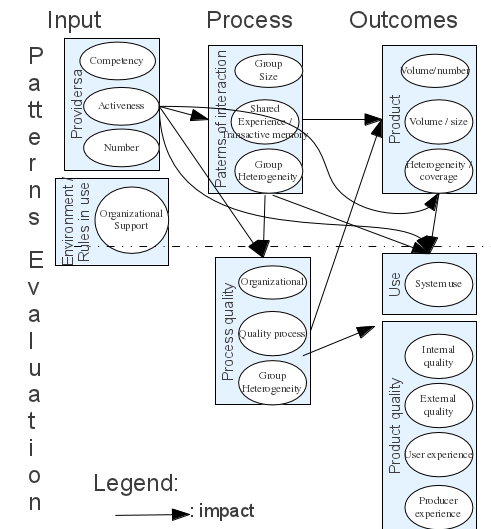
\includegraphics{Model_group_processes_open_communities_carillo_okoli}
\end{figure}

They did not explicitly take into account the retroactions, and did
not distinguish between the outcomes of the project and the specific
outcomes for the participants. One of the main differences between
these online projects (''communities'') and the other common good
productive communities is that the production outcomes (the pieces
of software, the Wikipedia articles) are available to all, when the
producers may have extra outcomes (and costs) to their involvement,
as we showed in \citet{JullienRoudautleSquin11}. 

For instance, \citet{CrowstonHowisonAnnabi06}, followed by \citet{LeeKimGupta09},
propose indicators to analyze the group production (they name ''system
creation''), and complete this model on two points. Relying on \citet{DeLoneMcLean92,DeLoneMcLean02,DeLoneMcLean03},
they proposed indicators to link the concrete outputs (here article,
in their case, open source software) to the user's satisfaction. In
their study, they also refer to \citet{Hackman87}, to show the importance,
as an output, of taking into account the producers (or contributors)
feedback, and the process of development to have a global view of
the outputs of such open online projects. They finally rely on \citet{Seddon97}
to extend Delone and McLean's model on the user side, with the concept
of ''perceived usefulness'', which echoes psycho-sociological studies
on the adoption of systems by users, such as Technology acceptance
model by \citet{Davis89} and its extensions \citep{Venkateshetal03}. 

Finally, Wikipedia is an example of a ``knowledge commons'' \citep{HessOstrom06b}.
These authors proposed a framework to understand the production of
such common, we present in figure \ref{fig:Institutional-Analysis-and},
page \pageref{fig:Institutional-Analysis-and}.

\begin{figure}
\caption{\label{fig:Institutional-Analysis-and}Institutional
Analysis and Development framework for knowledge commons \citep[p. 44]{OstromHess06}}
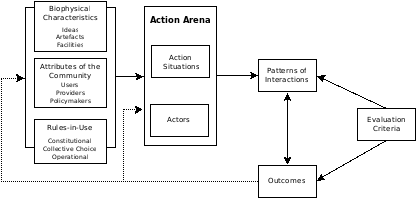
\includegraphics{Institutional_Analysis_and_Developement_framework_Hess-Ostrom}
\end{figure}

This leads us to a more global scheme (figure \ref{fig:Input,-process-and},
page \pageref{fig:Input,-process-and}), where inputs are the providers
as actors, the process the action arena (action situations) and mainly
the patterns of interaction, and the outputs, the outcomes, view from
different viewpoints, users, but also producers (providers in Hess
and Ostrom's terminology), and which can be seen as an extension of
the model proposed by \citet[p. 720]{ZhaoBishop11}. 

\begin{figure}
\caption{\label{fig:Input,-process-and}{Inputs,
process and outcomes of online open projects.}}
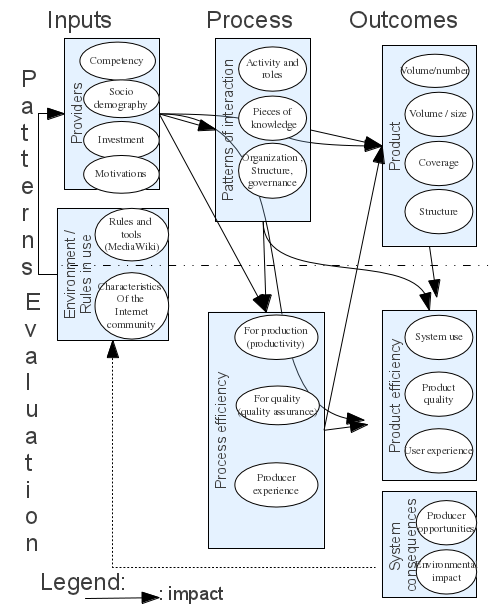
\includegraphics{New_model_of_group_processes_in_open_content_communities}
\end{figure}

Of course, as mentioned by the authors quoted, and what clearly appears
on Hess and Ostrom's framework, the outcomes influence the inputs.
The providers are given opportunities by their participation, leading
them to potentially involve more themselves in the project; the users
may also, by interacting with the system, become providers: for instance,
\citet{Lih04} shows that articles cited by the press see the number
of contributors increasing. We will come back to this point in the
conclusion of the article, but we argue that, before looking at how
this retro action loop works and impact the system, we have to understand
the system, which is the main goal of this work.

\subsection{The scientific production on Wikipedia.}

In concrete this means that a large part of the literature is out
of the scope of this article: neither the impact of the project on
the environment (the doted line in Figure \ref{fig:Input,-process-and}),
such as how it is used to comply professional tasks (by the students,
the researchers, the people in the industry), nor the analysis of
the propositions to improve the tools (using it on mobile, creating
a 3D Wikipedia), nor the use of Wikipedia as a database for information
retrieval test will be looked at here. This restriction does not provide
any restriction in terms of scientific scope (except for algorithm
research, data-mining, computational intelligence, semantic, information
retrieval), and we decided not to restrain our research to a particular
field as the topic is covered by various fields and as our goal was
to have an as extensive as possible view of the Wikipedia phenomenon. 
% * <nicolas.jullien@telecom-bretagne.eu> 2017-09-08T08:44:50.210Z:
% 
% From here, things have to be changed, according to what aer added
% 
% ^ <nicolas.jullien@telecom-bretagne.eu> 2017-09-08T08:45:44.621Z.
This is also the reason why we did not restrain to articles published
in journals, but added conference proceedings and books. However,
we restrain to papers published in English, French and Spanish as
we needed to understand the topics covered, and papers available before
February 2012.

We thus opted for a search strategy with high sensitivity \citep{DiestePadua07},
meaning that we searched with the keyword ''Wikipedia'' (or ''Wikip{\'{e}}dia)''
in the digital libraries (and not ''Wikipedia organization'', ''Wikipedia
evaluation'' or other terms which would have restraint the search),
in the title or keywords, but not in full text or in the summary as
we wanted that Wikipedia was specifically studied and not just an
example given in the text.

The original searches were conducted in December 2011 on Scorpus and WebofScience
databases. Bibliography for all the publications was stored in the
external bibliography system (CSV file and then Bibtex)\footnote{The query on Scopus was:

(TITLE(Wikipedia) OR TITLE(Wikip{\'{e}}dia) OR KEY(Wikipedia) OR KEY(Wikipédia))
AND (LIMIT-TO(DOCTYPE, ''cp'') OR LIMIT-TO(DOCTYPE,
''ar'')) AND (LIMIT-TO(LANGUAGE, ''English'')
OR LIMIT-TO(LANGUAGE, ''Spanish'') OR LIMIT-TO(LANGUAGE,
''French'')) AND (EXCLUDE(EXACTKEYWORD,
''Semantics'') OR EXCLUDE(EXACTKEYWORD,
''Information retrieval'') OR EXCLUDE(EXACTKEYWORD,
''Natural language processing systems'')
OR EXCLUDE(EXACTKEYWORD, ''Ontology'') OR
EXCLUDE(EXACTKEYWORD, ''Computational linguistics''))
AND (EXCLUDE(SUBJAREA, ''MATH'')) AND (EXCLUDE(EXACTKEYWORD,
''Artificial intelligence'') OR EXCLUDE(EXACTKEYWORD,
''Data mining''))}. We rejected introductions of panels, conferences, book reviews,
news flashes. We also deleted conference articles which were redundant
in the base, mostly because they had been presented in conferences
before been published in a journal, which let us with a bit less than
300 articles we read. Finally, we compared and completed the list
obtained looking at the list of the ''academic studies on Wikipedia''
maintained by the project itself\footnote{\url{en.wikipedia.org/wiki/Wikipedia:Wikipedia_in_academic_studies}}.

A first version were published in 2012. This version originates from this first version, and added references from there.

The rest of the article presents and discusses their findings, and
is organized accordingly to the framework proposed in figure \ref{fig:Input,-process-and}.

\chapter{Inputs}\label{cha:Inputs}
\input{03-input.tex}
\section{Environment, Rules in Use}\label{sec:EnvironmentRules}
Actually, speaking of the Wikipedia project can be viewed as a short-path,
as each language proposes a version, and has its own collection of
articles, more or less common with the English version.

% Cultural Environnement

\citet{HechtGergle10} studied 25 language projects and found that
the articles present in all the projects represent only 1\% of the
total, when 74\% of the articles were present in one language only.
For instance, \citet{CallahanHerring11} showed that the famous persons
for the English and the Polish Wikipedia are not the same \footnote{See also the differences in the periods of contribution, where some
language Wikipedias more contributed during the weekdays, such as
the English one, and other during the week-end (Japanese, for instance)
in \citep{YasseriSumiKertesz12}.}. 

\citet{PfeilZaphirisAng06}, analyzing the way French, German, Dutch
and Japanese contributed to the article ''game'', show a correlation
between Hosfstede\textquoteright s cultural dimensions \citep{Hofstede91,HofstedeMcCrae04}
and the way people perform different kinds of actions in the writing
of the article (number of correction, deletion, contributions). For
instance, there are statistically significant more courtesy behaviors
in the large Wikipedias that in the small ones (in terms of number
of articles) and in Eastern Wikipedias than in Westerns ones (\citealp{HaraShachafHew10},
in a comparative study of the English, Hebrew, Japanese, and Malay
Wikipedias). \citet{Stviliaetal09} compared the English Wikipedia
Feature Article quality process with the one of the Arabic and the
Korean Wikipedia. However the small size of the sample for the two
last (91 for the Arabic and 25 for the Korean), they showed that for
almost all the criteria used by the users to evaluate the articles\footnote{Well-written, Comprehensive, Factually accurate, Neutral, Stable,
Consistent with the style guidelines, Images, Appropriate focus and
length for the English and the Arabic, Well-written, Appropriate Length,
Neutral, Accurate, Links, Images for the Korean).}, there are strong variations between the three projects (at the date
of the dumps copy, June 2008). There are strong variation too, in
the representation of the knowledge (see, for instance, the study
by \citealp[part 6, p. 10]{Hammwohner07}, on how categories are subordinate
in various European languages). As early as 2005, \citet{Voss05}
noted a strong variation in the number of edit made by anonymous between
languages Wikipedia (10\% in the Japanese one, and 40\% in the Italian
one at the end of 2004), whereas the number of edit by people distribution
was quite similar. Some projects may have specific difficulties, making
the path of evolution barely comparable to the others, such as the
Chinese Wikipedia, which has had to solve the conflict between different
writing forms \citep{Liao08}, or small number of speakers Wikipedia,
which are quite empty of real articles, as shown by \citet{vanDijk09}.
This author also show the importance of the Internet access, but also
of the number of people able to translate articles from the English
to explain the difference in Wikipedia growth\footnote{On that aspect, he relied on the analysis of the Indonesian Wikipedia
made by \citet{SoekatnoGiri05} }, a result also stressed by \citet{Stviliaetal09}. Finally, as \citet{LiuIyer07}
pointed out, these variations may be also due to variations in age
and scale of the projects. As \citet{MarwellOliver93,OliverMarwellTeixeira85}
explained, in collective projects at the initial stage, people are
few and efforts costly, in the diffusion phase, the number of participants
grows as their efforts are rewarding, but with increasing need for
coordination, and the mature phase, some inefficiency may appear as
the contributors are more numerous than the work needed \citep[note that this has been empirically tested in the case of open online communities by][]{Alluvattietal11}.
if until 2006, and according to Wales, the English Wikipedia was written
by a small group of editors (talk at Stanford University in 2006,
cited in \citealp{Swartz06}), as early as 2006, \citet{Burioletal06}
showed that there were some indications of a permanent regime (they
call ''maturity''): for instance the constance of the average edits
per users, or the ''high correlation between PageRank and indegree,
indicating that the microscopic connectivity of the encyclopedia resembles
its mesoscopic properties'' (p. 8). \citet{Suhetal09} confirmed
this slowdown for the English Wikipedia. \citet{LamRiedl11} confirmed
that the English Wikipedia's production follows a S-shaped curve.

But what these various in projects have in common that healthiness
of a language project depends on the characteristics of the Internet
community (especially the number of Internet users, and the wealthiness
of of the population, according to \citealp{Rask08}), and on the
people's competencies \citep{GlottSchmidtGhosh10}, especially the
number of tertiary educated people within the population \citep{CrowstonJullienOrtega13}.
The global structure of the project, measured as a network, the nodes
being the articles and the links the links between the articles, seems
also to be the same, in terms of ''degree distributions, growth,
topology, reciprocity, clustering, assortativity, path lengths, and
triad significance profiles'', at least for the main projects \citep{Zlaticetat06}.
People also seem to contribute during the same period of time of the
day (between 1pm and 11 pm, still in \citealp{YasseriSumiKertesz12}).
Finally, \citeauthor{ZhaoBishop11}'s Delphi study (2011 p. 725),
points that the factors underlined by Wikipedia researchers to explain
Wikipedia's success are, in addition to its success, the rules in
use (especially the ones which promote communications) and the technical
structure which supports these rules and facilitates the editing.

% Environnement technique

As pointed out by \citet{HessOstrom06b}, as by the actor network
theory \citet{AkrichCallonLatour06,Latour05}, the artifacts, or the
tools used by the online communities are important to understand how
this community can work. Or, to quote\citet[p. 6]{NiederervanDijck10},
\textit{''Wikipedia {[}is{]} a gradually evolving sociotechnical
system that carefully orchestrates all kinds of human and non-human
contributors by implementing managerial hierarchies, protocols and
automated editing systems''}. Two tools seem to be of particular
importance to understand what Wikipedia is: first of all, the program
allowing to edit and manage the contributions, the MediaWiki. Several
structuring features of the Wikipedia collaborative organization are
due to this software \citep{PrasarnphanichWagner09}, such as the
collective editing, but also the existing of a talk page for each
articles, or the way links are made between articles and to the exterior.
This tool suffers certain limitations, from a content management orthodox
point of view, according to \citet{Doyle08}: there ''are clueless
about today\textquoteright s content management best practices like
content reuse, modularity, structured writing, and information typing''.
But as emphasized by \citet{Ciffolilli03}, in a transaction cost
theory based analysis of Wikipedia, ''Wiki technology in a way literally
cancels transaction costs for editing and changing information''.
This is a bit optimistic, as people have to understand how the changes
are stored and still have to discuss to content (see the section \ref{cha:Process,-or-the},
page \pageref{cha:Process,-or-the} on that aspect), but it surely
drop this cost \citep[p. 252]{RafaeliAriel08}, and also drop the
cost of degradation, or ''graffiti attacks'' \citep{Ciffolilli03},
as the tool keeps memory of the former versions and makes it easy
reversing. It also helps people, and especially the editors, in the
organization and in the structuring of their tasks \citep{Sundin11}.

However the importance of this wiki-based technical platform \citep{NiederervanDijck10},
it seems that, as the project has grown up, the socio-technique community
evolved ''from an informal trust-based community with few formal
roles to a socio-technique community where the social mechanisms,
and not the software architecture, supports knowledge management processes''
\citep{Jahnke10}. Even if it seems paradoxical, this is well illustrated
by a second software tool which has gained growing importance with
the success of Wikipedia, the bot. Because, a explained by \citet[end of p. 5 and following]{Geiger11}:
''Bots, like infrastructures in general, simultaneously produce and
rely upon a particular vision of how the world is and ought to be,
a regime of delegation that often sinks into the background {[}...{]}''

% Transition to the second tool, the bots

Bots are responsible for most of the publications of articles in endangered
language Wikipedias (\citealt[p. 12]{NiederervanDijck10} based on
\citealp{Rogersetal08}), resulting that most of these articles are
empty \citep{vanDijk09}. In the same time, still as shown by \citet{NiederervanDijck10}
on the list of the USA towns, the automate creation of articles facilitates
the completion of these articles in the future. The role played by
these automate tools is well illustrated by \citeauthor{GeigerRibes10}'s
analysis (2010) of the vandal fighting, and of the role played by
software in this task: in a comparison with the analysis of ship navigation
by \citet{Hutchins96}, they show how these tools implement human
decision facilitating their execution (the detection of task considered
as vandalism, or the automatic and comprehensive creation of a set
of information) and their management by automating the rules (gradation
in the sanction, formated messages), making these tasks ''mundane''.
But still pointed out by these authors, the definition of vandalize
and the punishments remain a moral choice, and the humans implement
the rules by programing these tools. Thus, these tools also are discussed
\citet[end of p. 5 and following]{Geiger11} ''\textendash{} that
is, until they do not perform as expected and generate intense controversies''.

% Rules in use.

These rules are numerous, increasing in number and complexity \citep[analyzing the English Wikipedia's rules]{Butleretal08},
and ranging from the the more formal and explicit (intellectual property
rights) to the more informal. 

First of all, it must be stressed that, as for software, articles
are protected by copyright laws, and that it is this protection which
grants the producer to license (in the Latin sense, authorize) the
user to use it. Here, this protection is used to ''copyleft'' the
use, to quote Stallman, but it comes also with obligations. The ''Creative
Commons Attribution-ShareAlike'' License, used for Wikipedia, allow
to use, to change, but if redistributed, the work built upon the article
has to be redistributed under the same terms and conditions\footnote{\url{http://creativecommons.org/licenses/by-sa/3.0/}}.
If this protection is juridically efficient is matter of debate (see\citealp{Wielsch10},
on that question), but this frameworks the vision people have about
the project and of its openness. Another legal based characteristics
of Wikipedia is that the name is a registered trademark of the Wikimedia
Foundation (non-profit organization), which also owns the technical
infrastructure which operates the service (servers). So, if this foundation
does not own the content, its own the right to ultimately decide what
can be posted under the name of Wikipedia and on its server, and its
board is only for a part elected by the participants in Wikipedia\footnote{\url{http://wikimediafoundation.org/wiki/Board_of_Trustees}}.
Quite surprisingly regarding their importance, especially in the open
source world, we can not find study of how Foundations manage open
online communities \citep[chapter 6, mentions this point however and gives a good start for Wikipedia.]{Reagle10}.
It is however clear that the leaders of these projects play an important
role in defining its goals and orientation (see \citealp{CrowstonHeckmanMisiolek10}
for an analysis of this aspect), especially in the case of Wikipedia,
where one of the two founders, Jimmy Wales, gave the vision \citep[chapter 1]{Reagle10}
and is still considered as the leader of the project, is the ultimate
decision maker \citep[chapter 6, which deals with Wikipedia leadership]{Reagle10}
and has a permanent seat in the board of trustees as founding member.

He is at the origin of the tables of law of the project, the ``five
pillars'' of Wikipedia\footnote{For the English: \url{http://en.Wikipedia.org/wiki/Wikipedia:Five_pillars},
but they are available in practically any language supported by the
project.}, defining the product (online encyclopedia) and its scope (neutral
point of view, no original research, accuracy, which are the three
core policy guiding the organization, according to \citealp{Reagle10}),
the producers and the users (anyone), and the process of production
(interaction and good faith), knowing that, as every project organization,
it has to be adaptable (no firm rules). \citet{CardonLevrel09,Cardon12}
propose a deep analysis of these explicit and implicit rules, showing
that these rules aim at involving any participant in the monitoring
and discussion of others' contribution, designing a procedural organization
(we will come back latter to this point). In other words, this organization
would be an attempt to create a ''supportive environment'' (\citealt{Reagle10b},
basing on \citealp{Gibb61}), i.e. an environment which privileges
''description (vs evaluation), problem orientation, spontaneity,
empathy, equality, provisionalism''. However, this also means that
the the foundations of the organization are constantly renegotiated
by the people (and by their behavior), leading ambiguity to be ''at
the heart of the policy process on Wikipedia'' \citep{MateiDobrescu11}.
It works because rules are mainly integrated by the persons in charge
(this is part of the process of involvement into the project), which
allows in the same time the maintaining of a common goal (the ideal
of consensus building and discussion) and the growing decentralization
of the day-to-day decisions due to the growing size of the project
\citep{ForteLarcoBruckman09}.

And when a very deep conflict appears, such as the case of the \textit{Jyllands-
Posten Muhammad Cartoon Controversy} \citep{MorganMasonNahon11} it
seems that the appeal to the values-in-practice, i.e. freedom of information
over multicultural inclusiveness (ibid, p. 7), thus to the common
rules, is a very powerful mean to gain the decision.

% Conclusion on that part, and history of the project.

The question is then to understand how this system is organize to
attract and retain these people, make them collaborate, and deal with
the growth of the population. As in many situations, the studies balance
between two positions: exploiting the data available, and the fact
that they are complete on the contribution, to provide general global
results on the participants, the products and the process, or deepening
the understanding beyond what is visible, thus trying to collect new
data, via exploratory methods, and compensating the loose in representativity
by a better understanding of the why or the how people do things.
Of course both are needed and complementary but, in general, we will
present the more global studies first, to have a global picture.
\section{Why do they participate?}\label{sec:Why-do-they-participate}

As \citet{PrasarnphanichWagner11} showed, Wikipedia is an aggregation
of contributors with varying levels of resources and interests, verifying
in that aspect too the fact that it follows the critical mass theory
\citep{MarwellOliver93}\footnote{For a formal model of this phenomenon, see \citet{Rahman08}}.
Most of the studies we read, minus one, looked at the motivations
to do positives things participating in Wikipedia. Quite strangely,
we did not find any study on the reasons for leaving Wikipedia, while
they would be interesting to understand how the contribution and the
benefits it brings change, but also, if it is possible, to prevent
these disaffections. Even if, according to the authors, the study
is preliminary, \citet{OrtegaIzquierdo-Cortazar09}, using survival
analysis techniques, showed that the mean time of participation to
the encyclopedia is between 200 and 400 days for the top ten projects
(with a median between 75 and 200 days), quite an important turnover.

This single study not looking at the motivations to do positive things
is by \citet{ShachafHara10} and looks at troll makers' activity.
It shows more social disorder than real motivations. However, these
activities impact on the information available (we will discuss more
this aspect in section 4) and it would be interesting to better understand
how to cope with these behaviors. It relayed on indirect information
about the four trolls they followed, because it was difficult to enter
in contact with them, as they hide their real identity. But this is
a common difficulty of the studies working on Wikipedians' motivation.
It very hard to be accurate in the same time on what people do and
why they do it, as these pieces of information come from different
origins, because there is few internal information on the participants'
skills, sociological background or motivations: \citet{Lametal11}
used users' page gender box and preference setting, for gender studies,
and report a gender information rate of only 6.5\% for editors (in
the English Wikipedia)\footnote{Even if \citet{Ashton11}, in a theoretical work, argues that the
whole editing and contributing activity is the signature, or the ''wikidentity''
\citep[term from ][]{MallanGiardina09} of a person in Wikipedia and
should be studied as so.}. 

So, most of the studies collected external data, via surveys, which
are hard to connect with an IP number or a Wikipedian login, in order
to link them to the internal data about participation. However this
difficulty, the studies available provide with a good understanding
of the characteristics and of the motivations of the participants.

\citet{GlottSchmidtGhosh10} surveyed Wikipedia users (and producers)
and measured their competency by the level of study, and by computer
skill, and their activeness by the time spent on Wikipedia. Another
option for activeness would be to measure the time spent by the participants
(users and providers), but this has not been done as far as we know.
The quality and the representativeness of these declarative data are
hard to verify. However, what these surveys tell us is that contributors
are of higher level of education, mostly male, older in mean that
Wikipedia users, and that mastering basic computer skill matters to
explain contribution\footnote{\citet{CollierBear12} relied on the English version of Glott et al.'s
survey to study the reasons why female Wikipedia users participate
less. Their explanation is that the encyclopedia is a conflicting
environment, and that these users have a lower confidence in their
expertise.}. According to \citet{LiangChenHsu08}, an for the Chinese Wikipedia
administrators they surveyed, having more personal time, weaker social
belongings, or longer Internet surfing time, increase the motivation
for being administrators. When the gap is bridged, the socio-demographic
variables are significantly less explaining of the difference between
contributors: there is, for example, no significant gender difference
in editing between registered Wikipedians \citep[in the English Wikipedia,][]{Antinetal11}. 

In addition to socio-demographic and skills variables, and still using
the survey method, \citet{Amichai-Hamburgeretal08} showed that psychological
characteristics such as agreeableness, openness, or conscientiousness,
are variables to take into account to explain the contribution to
Wikipedia. Focusing only on registered users, \citet{YangLai10} proposed
four types of motivation to explain this involvement: intrinsic (internal
satisfaction such as the pleasure or the fun to contribute, but also
the satisfaction to help by sharing their knowledge, which seems very
important for the most involved participants, according to the results
of a survey amongst Wikipedia administrators by\citealp{BaytiyehPfaffman10}),
extrinsic (image improvement, professional status improvement), external
self-concept-based (recognition by others and especially by peers,
tested by \citet{ZhangZhu11} on the Chinese Wikipedia), and internal
self-concept-based (acting consistently with their vision of themselves).
According to their study, self-concept-based motivations explain the
most the involvement, followed by intrinsic motivations (personal
enjoyment). This is consistent with a precedent study of Wikipedians'
motivation by \citet{Nov07}, which proposed the same methodology
and the same items.

However these global results, an important point is that the motivations
vary over time \citep{ForteBruckman05,Bryantetal05}, and that if,
for the most involved the recognition from the peers ('credit') is
an important motivation (ibid), as is the sense of mission (\citealt{LiangChenHsu08},
basing on a survey of Chinese Wikipedia administrators), for most
of the (small) contributors, the will to fix mistake is the principal
motivation, making these people not strongly committed to the project
\citep[relying on a survey of Japan Wikipedia contributors]{Kamataetal10},
a result \citet{DejeanJullien15} also found for the French Wikipedia
contributors. Using a qualitative methodology (20 semi-guided interviews),
\citet{Antin11} showed the large gap between readers (or occasional
contributors) and regular ones, especially regarding the feeling of
being part of the Wikipedia ''community'' and how this may refrain
from participating. This is explained by the fact that there is a
process of acculturation to Wikipedia: the future contributors are
firstly readers ''dipping their toes in to passively participate
while learning more about a complex system'' (\citealp{AntinCheshire10},
but surveying only US college students), even if the quicker the process
is, the greater the chance people become active contributors are (\citealp{DejeanJullien15},
surveying French Wikipédia's users and contributors, \citealp{PancieraHalfakerTerveen09},
analyzing registered contributors' trajectories). This would means
that the motivations to participate are more individual and internal
and are present since the beginning\footnote{\citet{PrasarnphanichWagner09} defended the idea that ''altruistic''
motivations prevail in Wikipedia, which seems going against this analysis.
But in their study they surveyed 60 very involved Wikipedians, so,
according to what was said, people for who the sense of the community
is the stronger. And the majority of their respondents had mixed motivations.

Regarding the presence of the motivations since the beginning, in
addition to \citet{PancieraHalfakerTerveen09,DejeanJullien15}, already
mentioned, a survey of students from U.S. universities contributing
to the Wikipedia content as part of their course work showed that
''intentions to continue contributing are influenced by the initial
attitude towards the class'' \citep{Zubeetal12}.}. 

In other words, as for open source \citep{LakhaniWolf05,Shah06,Scacchi07}
or professional communities \citep{JullienRoudautleSquin11}, this
may be an illustration of the idea of a path, or ''career'' in the
community \citep[in the sens given by][]{Becker60,Becker63}. To skip
from correcting a mistake to becoming a regular contributor, or an
administrator, would be an additional commitment, which would occur
for reasons developed during the attendance of the project as the
development of this sense of ''community'', i.e. the individual
acceptance of the rules of the organization, as showed by \citet{Pentzold10},
on his study of the meaning of the term community by the very involved
participants of the Wikipedia-1 mailing list (the surveys by \citet{ChoChenChung10}
of 223 English Wikipedians, by \citet{Hoetal11} on the Chinese Wikipedians,
and by \citet{SchroerHertel09} on the German ones all found a link
between this ''sense of belonging'' and the will to contribute).
\citet{KitturPendletonKraut09} also showed how the people modify
their practices of contributing when integrating the Wikiproject,
toward more administrative tasks, according to the group requirement.

This leads to the definition of the activities and the outputs of
this group, or, said differently, the patterns of interaction.

\chapter{The process(es), or the patterns of interaction.}\label{cha:Process,-or-the}
On the contrary, Wikipedia allows to access to a complete set of data
about the articles, their evolution, the people who contributed to
them, but also to the discussions which occurred before, during and
after the contributions. The articles exploring and exploiting this
fascinating set of data to better understand how people interact in
such an information system to product a public knowledge are mainly
threefold: first, the articles focusing on people and on their actions,
describing the activity and assessing roles from this activity; second,
the articles looking at the ''product'', the article; and third
the process of creation of such pieces of knowledge, with some works
looking at the other pieces of knowledge created in Wikipedia (mainly
the discussion pages). In general, the studies looking at the global
organizational structure rely on statistical analyses of the variables
present in the databases (Dump). Following the seminal work of \citet{KorfiatisPoulosBokos06},
most of these studies use social network analysis techniques, the
nodes being, usually, the people, and the arcs the fact they contribute
to the same article or the same talk page. On the article side, the
node are the articles and the arcs the fact that they refer to each
others (sometimes those two approaches are mixed). When seeking to
improve the processes of collaboration, scholars privileged usually
more narrowed sets of articles, their evolution and the one of their
talk pages, but deepening the analyses of the content produced.

\citet{Slattery09} used a quite similar segmentation and provides
a nice first approach to the main characteristics of these patterns,
approach we are developing here.


\section{The contributors, their activity and roles (what they do).}\label{sec:The-contributors,-activity}

This part is a perfect illustration of the too kind of studies found
on Wikipedia. There are, actually, few studies looking at the contributors
as deeply as \citeauthor{Sundin11}'s one (2011), which presents the
day-to-day life of Swedish Wikipedia editors and underlines the importance
of the tool (Mediawiki) and of the basic rules structuring the tasks
(vandal fighting, verification of sources, improvement of sourcing...)
On the other side of the spectrum, \citet{AnthonySmithWilliamson09}
proposed a quite macroscopic, but also more comprehensive point of
view: they separated the contributors into two groups (registered
and non registered), and analyzed their contribution for the whole
English Wikipedia. If they couldn't infer much about the number of
people in each groups, they stressed the importance of those anonymous,
as they represent, for instance, 20\% of the contributions that remain
in the Spanish Wikipedia \citep{DruckMiklauMcCallum08}. In other
words, if most of the best contributions in terms of quality is done
by registered users and by a small subset of the whole contributors,
a significant number of anonymous users also do provide quality content
\citep{Javanmardietal09}.

% Activity and roles

As explained before, we will first look at the studies relying on
the data provided by the project, thus giving a global and comprehensive
view of the participants, or at least of the \textquotedblright authors\textquotedblright ,
defined as the people registered in Wikipedia and having done a contribution,
because their registration makes it possible to follow their activity
(thanks to the data stored in the MediaWiki table \textit{user\_groups}).

Regarding the activity of each of these registered authors, it has
been shown that the number of article per authors follows a power
law \citep{Voss05}, like in open source and in scientific publication
(ibid and \citealp{Maillartetal08,ArafatRiehle09} regarding open
source), something known as the Lotka's law (ibid), as does the number
of contributions per person, in all the main language projects \citep{Kitturetal07b,OrtegaGonzalez-BarahonaRobles08,Ortega09,Javanmardietal09,Zhangetal10}.
However, it seems that the percentage of contribution coming from
the users having privileges (administrators of Wikipedia) which are
the biggest contributors, is decreasing with the age of the project
\citep{Kitturetal07b,Ortega07,Ortegaetal09}. In the other hand, their
contributions dominate what people see when visiting Wikipedia \citep{Priedhorskyetal07}:
''The top 10\% of editors by number of edits contributed 86\% of
the PWVs {[}persistent word views{]}, and top 0.1\% contributed 44\%
\textendash{} nearly half! The domination of these very top contributors
is increasing over time.'' (p. 5) \citet{LaniadoTasso11}, completed
this point, using English Wikipedia's dump data, finding evidence
of ''the presence of a nucleus of very active contributors, who seem
to spread over the whole wiki, and to interact preferentially with
inexperienced users''. 

This apparent paradox is easy to understand: as Wikipedia, and especially
the English language project, became bigger, the editing tasks have
increased in complexity (see \citealp{FongBiuk-Aghai10} for a proposition
of classification in terms of semantic complexity of these various
type of edits), and have increased also the proportion of non-editing
tasks. In other words, participants' types of activity have multiplied.
Behind the writing, which can be seen as the emerged part of the iceberg,
but also the most important part, for an encyclopedia, are the actions
leading to the writing (coordination tasks, discussions on the topic
of the project, etc.) 

Regarding the edits, \citet{Adleretal08a,DruckMiklauMcCallum08} may
be the ones who proposed the more complex evaluation of authors' editing
contributions, based not only on the volume of add-ons, but also of
their persistence (what they call the longevity). The interest of
this statistical method, which uses dump data, is its ability to be
implemented for the all set of authors in a project. It made it possible
to identify bots and vandals \citep{Adleretal08a}, and provided insights
to \citeauthor{AnthonySmithWilliamson09}'s arguments (2009) that
anonymous contributions are important.

Another part of the literature looks at these other activities, not
only at the contribution to article writing, but also to discussion
and project pages, user talk pages, leading to a typology of participants'
behavior, or ''social roles''\footnote{For a study of social roles in Online Communities, in addition to
\citet{Welseretal11}, which rely on Wikipedia, see \citet{Gleaveetal09}.}. This can be seen as a decrease of the quantitative scope (exploitation
of the data) toward more qualitative data, in order to increase, to
deeper the qualitative understanding of the practices (exploration).
We will organize the presentation of the papers this way in the rest
of this part.

\citet{UngDalle10} emerged a ''project leader'' role, based on
project page editing activity (a project leader is the one who does
more than 5\% of the edits on a project page). They found a positive
correlation between the coordination tasks (editing activities in
the talk pages) and the contributions to the article of these leaders. 

\citet{Ibaetal10} looked at a very small set of articles and people,
but went deeply into the interaction between those people in the contribution
(edits) and then in the talk pages. They used social network analysis,
the nodes being the persons and the weighted edges the number of time
author B contributes to the same article as author A. Looking at the
activity in the talk pages of four very active editors in the start
and the building of quality articles (''coolfarmers in their terminology''),
they found two types of patterns: ''the mediators, trying to reconcile
the different viewpoints of editors, and the zealots, who are adding
fuel to heated discussions on controversial topics''. They also identified
''egoboosters'', i.e. people who mainly use Wikipedia to present
themselves, which, if being done by adding entries to the encyclopedia,
is against the rules. 

As for other open source communities such as Python \citep{BarcelliniDetienneBurkhardt08},
\citet{Harreretal08,Halatchliyskietal10}, both investigating sub-projects
(domains) of the German version of Wikipedia, showed the importance,
for the construction and the structuring of the knowledge in Wikipedia,
of the ''boundary spanners'', in the sense given by the Sociology
of Translation \citep{CallonLawRip86,AkrichCallonLatour06}, i.e.
those people who are at the intersection of several domains of knowledge
and because they have a broader view ''are not only responsible for
the integration of knowledge from a different background, but also
for the composition of the single-knowledge domains. Predominantly
they write articles which are integrative and central in the context
of such domains.'' 

\citet{Huvila10}, using a ground theory approach via an online opened
questions survey to contributors, proposed a classification in five
types for the contributors, according to their activities and to the
way they find their information (table \ref{tab:Groups-of-Wikipedia}).

\begin{table}
\caption{\label{tab:Groups-of-Wikipedia}Groups of Wikipedia contributors according
to a qualitative analysis of the research data, from \citet{Huvila10},
table 1.}

\begin{tabular}{|c|>{\centering}p{14cm}|}
\hline 
Group & Description\tabularnewline
\hline 
\hline 
Investigators & Contributions relate to personal interest or hobby related area (of
expertise) based mostly on news sources, popular scientific or fact
literature and/or visiting the local library {[}...{]} They represent
the hard core of contributors who start articles and make considerable
contributions to existing ones. 

\textit{Members of the group were mostly graduates, professionals
working on topics other than those to which they are contributing.} \tabularnewline
\hline 
Surfers & Contributions are based on easily findable sources available on the
net. Surfers spend their time on using search engines and finding
fitting material for articles. Their personal interest on the topics
they are editing is similar to the group of investigators, but they
do not investigate the same sources of information.

\textit{Surfers are primarily secondary school educated, undergraduates
and professionals.}\tabularnewline
\hline 
Worldly-wise & These contributors tend to focus on topics relating to their own sphere
of experience and knowledge. They do not tend to seek information
explicitly for their Wikipedia contributions and tend to rely on serendipitous
information seeking and information discovery. 

\textit{Background and the level of experience vary.}\tabularnewline
\hline 
Scholars & Contributions on an academic or professional area of expertise. 

\textit{The archetypal contributor in this small, but quite distinct,
group is a PhD student or a relatively young researcher who is contributing
on the topics related to their research.}\tabularnewline
\hline 
Editors & Some of the editors focus on administrative tasks, grammatical corrections,
correction of inconsistencies between articles, and another group
on translations from other language versions of Wikipedia. They do
not generally seek information for their Wikipedia edits. 

\textit{The group was very small and rather heterogeneous in the present
study, but they shared, broadly speaking, a professional background
and a college level education. }\tabularnewline
\hline 
\end{tabular}
\end{table}

\citet{Welseretal11} directly referred to social role literature
and provided, in addition to a synthesis of \citet{Harreretal08,Halatchliyskietal10,Ibaetal10},
a complementary perspective of Huriva's classification, integrating
the social interactions (the discussion activities). They looked for
''structural signatures social attributes of actors'', i.e. the
actions taken, but also the network of interaction, and the social
interaction, especially in the talk pages, in the user pages, and
in the user talk namespaces. It is a rather exploratory survey, based
on qualitative analysis for identifying roles, and studying the differences
in action, network, social interaction of these roles using dump data.
It does not provide a lot of extra information about the first four
type of contributors, beside the fact that they pointed out that some
of these contributors, they named ''substantive experts'', ''invest
time in fact checking and article talk to discuss details of articles''
(p. 4). But their work seems to indicate that Huriva's ''editors''
can be split into three sub-groups, ''technical editors'', ''make
numerous small changes to content pages, frequently specializing in
a particular type of problem'' and with few presence in the talk
pages (p. 7), ''counter vandalism editors'' (ibid) who correct vandalized
pages and post warnings in vandal's user pages, and the ''social
networking editors'' (ibid), who invest few in the editing, but a
lot in the social interactions, the community building. 

%Here also is the introduction of the time, the evolution of the people

Of course, as the motivations vary, the level or type of contribution
may also vary among time. However, \citet{PancieraHalfakerTerveen09},
using internal data of the English Wikipedia, with time series, and
\citet{DejeanJullien15}, surveying French Wikipedia contributors
reached the same conclusion: the level of participation strongly depends
on the first contributions to the project. \citet{AntinCheshireNov12}
went a bit further, showing that not only the level of activity, but
also the type of tasks can be statistically predicted by the first
contributions. But this does not mean that everybody follows the same
path. For instance, \citet{OkoliOh07}, looking at English Wikipedia
contributors, showed that people having lots of participation in various
articles (they assimilate to ''weak links'', in a \citet{Granovetter85}'s
framework) are more likely to become administrator (to have administrative
rights) than those more focused on a sub-set of articles and talking
with a small subset of people (and then developing strong(er) links).
In addition to this, it seems that the administrators are not among
the most active contributors to the articles, and that their share
in the total contributions is decreasing over time, at least for the
English Wikipedia \citep{Ortega07}. This lead \citet{Zhuetal11},
relying on \citet{Bryantetal05}'s study, to propose two main careers
for the people, coherent with Okoli et Oh's findings: from non-administrators
to administrators and from non-members to Wikiproject regular members
to Wikiproject core members (figure 1, page 3433). On that aspect,
\citet{AntinCheshireNov12} confirmed that people involved from the
beginning in more diverse revision activities are more likely to take
administrative responsibilities.

These findings reinforce the perception that there is an à la Becker
career for contributors, and different paths of participation, with
a learning process (future contributors are firstly readers ''dipping
their toes in to passively participate while learning more about a
complex system'', according to \citet{AntinCheshire10}, surveying
a population of US college students). As it is the case for the involvement
in other communities of practice like open source (see, for instance,
\citet{FangNeufeld09} and \citet{SchillingLaumerWeitzel12}) there
is a period of apprenticeship, via legitimate peripheral participation
\citep{LaveWenger91}, as showed by \citet{Bryantetal05}. 

These last paragraphs question the existence of an ''efficient''
structure of interaction to produce the articles and of an ''efficient''
process of inclusion. But before looking at these interactions, we
have to better understand what is produced, the pieces of knowledge
that are the articles and the articulation between them.

\section{Pieces of knowledge, articles, and global structure.}\label{sec:The-pieces-of-knowledge}
Being the core of the project, it is not surprising that this topic
is one of the first to have been studied. The studies can be split
in two, the firsts looking at the articles in general, the seconds
studying one specific kind of articles, the Feature Articles, which
are considered by the projects as the best articles (their intrinsic
quality is, however discussed \citep{Lindsey10}, and the arguments
of quality to qualify an article as Feature Article (FA) varies from
one language to another, according to \citet{Stviliaetal09}, two
points we will come back to in the last section). As for the precedent
sub-section, we will start from the studies looking at the global
structure of the project (and relying on statistical analyses of the
dump data, for most of them), toward the analyses of the edition of
article, finishing with some remarks on the dynamics of interaction
behind this process.

\subsection{Structure of the project.}
\citet{Voss05} provided with the first global figures on the articles
(mostly on the German Wikipedia), showing a lognormal-like distribution
in their size (ibid, Figure 3, p. 6), which stabilizes when the project
gets a certain size (even if the articles' mean size is growing) and
that the number of distinct authors per article follows a power law
(Figure 4, p. 7), as the numbers of ingoing and outgoing links (ibid,
Figure 7, p. 9). \citet{NazirTakeda08} found globally the same results
on the English Wikipedia for the number of users per article. \citet{Capoccietal06}
looked at the links between articles and found that the structure
of these links is closed to the World Wide Web's one and found ''a
scale-invariant distribution of the in and out degree''. This led
them to conclude that ''Wikipedia growth can be described by local
rules such as the preferential attachment mechanism\footnote{From \citet{BarabasiAlbert99}, this mechanism says that the more
popular articles (in terms of contributors, links...) are, the more
likely to increase their popularity is. }, though users, who are responsible of its evolution, can act globally
on the network.'' Note that this preferential attachment mechanism
has been proposed as an explanation by \citet[p. 9]{Voss05}. These
considerations have been summarized by \citet{WangJinWu09}, saying
that a small number of people is strongly connected to lots of people
and assures the coherence and the small world effect of the model,
whereas the vast majority aggregates around centers of interests and
is poorly connected. Also, the more popular topics (and central people)
are those who aggregate new people the more (\citealp{KeeganGergleContractor12}
gave an example of this phenomenon: looking at articles about plane
accidents, they showed that breaking news articles are those which
are the most likely to attract new editors, when experienced users
remained more focus on their own agenda and editing 'their' set of
article).

\citet{Zlaticetat06} did similar analyses on the main Wikipedia languages
projects and found that ''degree distributions, growth, topology,
reciprocity, clustering, assortativity, path lengths'' are common,
and defended the idea of an unique growth process. Finally, \citet{WangMaCheng10},
studying the categories (or tags) which define the pages, showed that
there is an obsolescence phenomenon, as if the categories followed
the actuality or that they are created when the articles and the topics
they refer to are created. 

One has to be very careful, however, to draw general conclusions from
the analysis of the global structure of the project. As shown by \citet{Silvaetal11},
who analyzed four sub-projects of the English Wikipedia (Biology,
Mathematics, Physics and Medicine). These sub-projects present very
different structures regarding the links between articles, with dense
links in biology and medicine and less in physics and Mathematics.
The reasons for these differences are not explicit, and more work
would be useful to understand if they are due to the internal characteristics
of the disciplines or to the internal organization of the Wikipedia
sub-projects. (We will come back to this point in the discussion on
the growth of the project at the end of this part).

We have not found any comparison with the other online encyclopedias
regarding the global structure (distribution of the size and of the
links of an article), a study which would be interesting to conduct
to see if Wikipedia is different on this aspect.
\subsection{Structure of articles edition.}
\citet{GorgeonSwanson09} studied one single article (Web 2.0), an
article edited by more than 1,000 different people, and showed that
the publication followed an S-curve pattern. Taking an actor network
theory perspective \citep{Latour05,AkrichCallonLatour06}, \citet{Swarts09}
showed how the building of an article, especially a polemic article
(clean coal), is a process of accumulation of facts, and of ''translation''
of arguments or proposals in facts, this accumulation of facts being
harder and harder to contest and thus to delete. It is partially confirmed
by \citet{Luytetal08}, who showed that ''a sizable number of error
edits occurs in the very first edit'' and if ''many more error edits
appear in the last third {[}part of the life of the article{]}, a
fifth of the errors {[}remaining{]} are attributable to the first
error edit.'' As early as 2004, \citet{ViegasWattenbergDave04} also
found that, in the English Wikipedia, there is a strong dependence
on the first edit for the global structure of the article. Finally,
\citet{Halfakeretal09} showed that ''the number of reviews a word
survives is a strong predictor of whether the edit that removes the
word will be reverted'' (p. 9). The question these articles raise
is how the negotiation around the facts is done, and what the structure
of the team needed to do it is, things we are going to analyze in
the next sub-section. \\

% FA articles.

Another important part of the literature looks at the characteristics
of the articles, and particularly of the articles recognized by the
producers as good (the Featured Articles, or FA). \citet{Luytetal08}
proposed a still actually categorization of the different algorithms
used to automatically retrieve the Feature Articles.

For instance, \citet{Lih04,Brandle05,WilkinsonHuberman07}, confirmed
by \citet{Ortega09}, found that after taking into account age and
visibility (using Pagerank as a proxy), those Featured Articles have
statistically more edits and editors. \citet{WohnerPeters09} refined
these analyses, showing that these articles are ''in general more
persistently edited than low quality articles and that on the other
side they have a stage of a high editing intensity in their lifecycles''.
(p. 7) 

\citet{Adleretal08b}, on the English Wikipedia, noted that ''incorporating
the authority of reviewers gives good and robust performance'' to
characterize FA articles. This authority is measured as evaluating
author's contributions life-length, based on the argument, brought
by \citet{Cross06}, that their persistence is a proof a quality (something
which is quite fragile, \citealp{Luytetal08} showed). \citet{Huetal07}
on a subset of articles, found the same result. \citet{Mcguinnessetal06},
based on the same idea as Pagerank, looked at the internal links pointing
to the articles (they named the ''trust ratio'') showed that Feature
Article are significantly more cited. 

Also, and coherent with the analyses done on the contributors, FA
articles have experienced editors participating to their redaction
\citep{SteinHess07}. More precisely, a fine tune of experimented
editors and fresh newcomers increases the likelihood for an article
to become FA \citep{RansbothamKane11}, which, in other contexts,
have been proven to be very important for group's creativity and efficiency
\citep[for instance, ][]{UzziSpiro05,Uzzi08}. \citet{WilkinsonHuberman07}
also found that these articles have more discussions on their talk
page, which is rather normal as, as pointed by \citet{ArazyNov10},
''processes for becoming a featured article explicitly require additional
coordination activities'' (p. 234).

But it seems that, in a first approach, the best indicators of an
Feature Article, at least for the English version \citep{Dalipetal09}
are the length and basic quality of the writing, as it is for open
source contribution, actually\footnote{\citet{HofmannRiehle09} found that for open-source, simple heuristics
are superior to the more complex text-analysis-based algorithms to
estimate the size and the importance of a commit in open-source projects.}: textual features related to length \citep[result already stressed by ][]{Blumenstock08},
structure and style (\citet{LipkaStein10} even obtained a better
result on FA identification with a machine learning approach on article
styles than \citeauthor{Blumenstock08}'s algorithm on length); and
those which count for the less, are the most complex features, such
as those based on link analysis.

This kind of analysis can also be done at portal, or subject level,
as did \citet{Poderi09}, with rather against-intuitive results, as
it seems from this analysis that subjects having more feature articles
(high density subjects in his terminology) have longer articles, but
less edit and contributors than low density subjects, while the ratio
between major and minor edits is the same in the two groups. It seems
also that there is more often a single major editor in the high density
subject articles. However, as stressed by the author, this study has
been done on a small subset of articles and should be extended to
confirm its results. \citet{Jones08} proposed an analysis of the
revision patterns of the articles applying for FA label, and showed
that the final structure of the article is very dependent on the first
one, editors tending to expend sentences, paragraphs and sections.
His study having been done on a small subset of the articles also
(10), he questioned the fact this unique revision pattern is global
or not, which seems to be the case, according to the studies done
on the whole set of articles.

\citet{Ibaetal10} proposed an explanation to these seemingly contradictory
results. According to them, there would be two types of FA (in the
English Wikipedia): (1) articles of narrow focus created by few subject
experts, and (2) articles about a broad topic created by thousands
of interested incidental editors. Considering the preferential attachment
mechanism, this phenomenon is self-maintaining as the more exposed
articles are, the more probable is the fact that people contribute
to them (a result studied by \citealp{RansbothamKaneLurie12}).


\section{The organization, structure, and governance of the project.}
\citet[p. 18]{KitturKraut08} noted that \textquotedblleft decades
of research in organizations show that communication as the basis
for coordination is especially important in tasks that are highly
uncertain, unconstrained, and subject to many changes\textquotedblright ,
as can be the construction of the content of an article (\citet{CardonLevrel09,Cardon12}
explained, in the particular case of Wikipedia, why and how the rules
in use are not always enough). This explains the importance of the
talk pages in the project, even if there are variations between the
projects (\citealp{Voss05} showed strong differences in the ration:
user talk over user pages, between the European projects (German 0.94,
Danish 0.88, Croatian 0.74) and the Japanese one, 2.51). \citet{PancieraHalfakerTerveen09},
quoting \citeauthor{Viegasetal07}'s result that over half of Talk
page comments are requests for coordination and 8\% are policy invocations
(2007), concluded that Wikipedia contains strong and supportive communities.
\citet{Butleretal08} also found that much of the explicit coordination
is managed through the Talk or discussion pages for the article in
question.

Not surprisingly, if taking into account Actor Network Theory \citep{Latour05,AkrichCallonLatour06},
studying these discussions, and especially the ''conflicts'', can
give explanations on the repartition of the work between direct contribution
to articles, vandalism fighting and discussion or negotiation of the
''point of view'', leading to mutual adjustments when the rules
are not enough to do so, but also of the brutal rejection of ''pathologic''
discussants \citep{Aurayetal09}. It is also a well know issue for
distant (virtual) organizations \citep{HindsBailey03,HindsMortensen05},
both negative because it consumes people's time, and positive because
it can strengthen the community \citep{Francoetal95}\footnote{For a discussion of the cause of conflict, the way the Wikipedia organization
could avoid them and the need for a better understanding of the process
of conflict management, see the study of ''the bibliography of the
living persons in Wikipedia'' by \citet{JoyceButlerPike11}.}. We have not found any survey on the patterns of interaction, probably
because they will suffer from the same problem as the ones regarding
implication, and because of the already rich data available. These
surveys would be of help, however, to understand how people choose
the article they contribute to (topics, people working on it), and
their perception of the conflicts, and thus to deeper the understanding
of the structure of interaction the data analyses make apparent.

But before looking, thanks to the discussion pages (and the analyses
made on them), at the processes behind the life of an article (creation,
deletion, evolution, promotion), and at the managerial behaviors,
and to follow up the discussion started, we will start giving some
results on the who and the how of the construction of an article.
In a word, what a 'good' team to construct an article is.

\subsection{People, team and articles.}

\paragraph{People and articles.}

\citet{Halfakeretal09} found ''strong evidence of ownership behaviors
in practice'' in the production of an article, especially in the
articles designed as ''Maintained'', according to \citet{Thom-SantelliCosleyGay09},
despite the fact that ownership of content is discouraged. And, even
if less geographically situated than Flickr contributors \citep{HechtGergle10b},
Wikipedia ones can often be associated with ''relatively small geographic
regions, usually corresponding to where those users were born or where
they presently live. Also, for many users, the geographic coordinates
of pages to which they contribute are tightly clustered'' \citep{LiebermanLin09}.
Finally, \citet{HardyFrewGoodchild12} geolocalized IP addresses for
the anonymous contributions to geotag articles in 21 language projects
and concluded that ''the likelihood of an anonymous contribution
to a geotagged Wikipedia article exponentially decreases as the distance
between the contributor and article locations increases''. All these
behaviors are coherent with the findings of \citet{Zhangetal10} who
concluded that it seems that people involve themselves on a very specific
themes, at article level, rather, than, for, instance at domain level,
after looking at a subset of articles on terrorism and comparing them
to the Terrorism Knowledge Base. As pointed by \citet{Thom-SantelliCosleyGay09},
this focus, these ownership behaviors, are not bad per se, especially
in the first stages of an article where a small team seems to be more
efficient. But it can lead to overprotection and can decrease the
final quality of an article (see bellow the discussion on the form
of the team).

This does not mean either that there is no coordination at project
level or that people can not be asked to joint a particular project.
On the contrary, \citet{Zhuetal11} showed how the personal pages
are specifically used to do so. But this must be fine tuned: \citet{Choietal10},
also analyzing the messages on the personal pages, showed that welcome
messages, assistance written in newcomers' pages are quite effective
to improve their contribution, when ''invitations led to steeper
declines in edits.'' Other actions can also attract contributors
and structure the teams or, more precisely the discussions, such as
template message on the articles: \citet{Rossietal10} studied the
role played by NPoV (neutral Policy Violation) templates, which if
not made completely explicit by their analysis, seem to be used to
settle evidence of a latent conflict \citep{DenBestenetal10}, and
thus to attract the attention of the community on a problem which
has to be solved, whereas other template messages seem to be more
treated as simple messages.

These recruiting actions play a crucial role in the construction of
a ''good team'' for writing an article, which appears to be a congregation
of experienced people having already work together with new talents.

\paragraph{Form of the team.}

\citet{KitturKraut08} showed that explicit coordination (talk) is
more efficient when there are few editors, when implicit coordination
(few editors editors concentrate the main part of the edits when the
majority is peripheral editor) is more efficient when there are more
editors. They also found that explicit coordination is needed more
at the early stage of the article. In any case, there is a core-periphery
structure, similar to the one found in open source software production,
and things are easier when the core team people already know each
others: \citet{NemotoGloorLaubacher11} pointed out that ''the more
cohesive and more centralized the collaboration network, and the more
network members were already collaborating before starting to work
together on an article, the faster the article they work on will be
promoted or feature''. In the same time, \citet{ChenRenRiedl10},
evaluating diversity according to an evaluation of the interest of
the persons via their contribution, showed that ''increased diversity
in experience with Wikipedia increases group productivity and decreases
member withdrawal - up to a point. Beyond that point, group productivity
remains high, but members are more likely to withdraw''. Interestingly
for this theory, \citet[p. 22]{Tureketal10} showed, using Polish
Wikipedia data set, that in what they call ''good teams'', the level
of acquaintance is higher than for normal teams (people having discussed
in the talk pages) as is the level of trust (copy-pasting of existing
text when rewriting an article) and of distrust (deletion of text),
which can be seen as the level of creative work (if people delete
more that means that the consensus is reached more slowly, after more
evaluation of the proposals). This is true for FA, but also when articles'
quality is measured by external experts, as in \citeauthor{ArazyNov10}'s
article (2010), who estimated the impact of local inequality and global
inequality on the quality of the article: having a small team, very
committed (strong local inequality), improves the coordination (and
thus indirectly the quality), and having strong global inequality
(people very invested in Wikipedia and peripheral contributors) improves
the quality of the articles (of course, this work may be extended
to a bigger set of article to be confirmed). \citet{GomezKappenKaltenbrunner11}
also showed that ''once a comment on a Wikipedia article has been
originated, it will derive in a collaborative reciprocal chain between
a very reduced group of contributors'', indicating, and contrary
to the contribution to an article, an ''inverse preferential attachment
process'' for the discussions (p. 8). Finally, \citet{XuYilmazZhang08}
can be seen as a summary of these findings: using an agent simulation,
they retrieved these results, showing that more agents improve the
convergence and the quality of the article, especially if they are
more knowledgeable, and vandalism, if increasing the number of updates,
does not stop an article from being improved (it can be seen as test
which allows to question the team and eventually improves its production).

\paragraph{Conclusion.}

The conclusion can be led to \citet{Arazyetal11}, even if they focused
only on a very small subset of articles (96): ''(1) diversity should
be encouraged, as the creative abrasion that is generated when cognitively
diverse members engage in task-related conflict leads to higher-quality
articles''; (we will just add ''up to a point'' here) ''(2) task
conflict should be managed, as conflict notwithstanding its contribution
to creative abrasion can negatively affect group output'' (we will
come back to this point in the next paragraph); and ''(3) groups
should maintain a balance of both administrative- and content-oriented
members, as both contribute to the collaborative process.''

This echoes more general findings about the efficiency of groups.
As shown by \citet{UzziSpiro05} in the case of musical comedies,
and \citet{Uzzi08} in the case of a social network, for a creative
group to be successful, it needs to fine tune the level of newcomers,
for fresh ideas, in an already constituted group (for trust and common
sharing, or ''cohesion'', especially on what a good article is for
Wikipedia, as, according to \citet{ArazyNov10}, the fact to have
people having experience in the contribution in general, or, as we
named them before, boundary spanners, is even more important than
to have people who involve themselves in the production of the article).
Wikipedia seems to be another proof of this principle and it would
be interesting to calculate Wikipedia's ''Q''-level ''bliss point''.

% Transition

This Q-level may depend on the type of article, more specialized,
''narrow focused'', or more general: \citet{KeeganGergleContractor12},
comparing breaking news with historical articles on the commercial
airline disasters, in addition to find the same results as the articles
already cited about the link between quality and number of editors
or length of the article, showed that breaking news articles are more
often chosen by newbies, and that experienced users may avoid this
kind of article.

These studies on the structure help to understand what is needed to
make an article, but give few information on the making, of the life
of this article, and on the interactions needed for this making, which
is the subject of the following paragraph. 
\subsection{The life of an article: creation and deletion, redaction, and promotion.}
We will start with two main moments in an article life, the decisions
of deletion and of promotion, before looking at a larger-in-time process,
the cooperation around the article.

\paragraph{The decisions regarding an article.}

The editing arguments leading to these deletions are quite on line
with the rules of the project, as shown by \citet{WestLee11}, on
a corpus of one year deletions in the English Wikipedia: the non-respect
of the non-novelty rule, but also, the ones which ''present a legal
liability to the host (e.g., copyright issues, defamation), the harder
to detect, or privacy threats to individuals (i.e., contact information).''
If copyright issues are hard to discuss, the others are subject to
interpretation and the decision of deletion can be taken after a vote.
On that aspect, \citet{TaraborelliCiampaglia10} showed that there
is a ''herd effect'': ''an over- or under-expression of preferences
in the initial part results in an over- or under-expression in the
following'' (p. 3), which, according to the authors, can be due to
recruitment activities among voters' group, or as studied by \citet{GeigerFord11}
on the English Wikipedia, that the final decision remains to experimented
users, and that this expertise is recognized by the voters. \citet{LamKarimRiedl10}
analyzed the various elements impacting the quality of the deleting
decision and we reproduce their findings in table \ref{tab:Impact-of-structure-group},
page \pageref{tab:Impact-of-structure-group}.

% process of promotion of articles.

This mechanism is also apparent in the process of promotion of the
articles. \citet{KeeganGergle10}, who studied a corpus of 161 deliberations
(in a 3 month time frame), concluded that elite users ''fulfill a
unique gatekeeping role that permits them to leverage their community
position to block the promotion of inappropriate items. However, these
elite users are unable to promote their supported news items more
effectively than other types of editors.'' (on breaking news stories)

\begin{table}
\caption{\label{tab:Impact-of-structure-group}Impact of the structure of the
group on the quality of the decision regarding article deletion, from
\citet{LamKarimRiedl10}, table 3, p. 10.}

\begin{tabular}{|c|c|>{\centering}p{8cm}|}
\hline 
Hypothesis & Result & Description\tabularnewline
\hline 
\hline 
H1 Bigger-Better & Supported & Larger groups make better decisions, but with diminishing returns\tabularnewline
\hline 
H2 Recruit-Worse & Mixed & Biased recruitment leads to worse decisions under some circumstances\tabularnewline
\hline 
H3a Newcomers-Worse & Supported & Newcomer participation yields worse decision quality\tabularnewline
\hline 
H3b Diversity-Moderate & Mixed  & Diverse groups may make better decisions; no social categorization
effects were observed\tabularnewline
\hline 
H4 Biased-Admin-Worse  & Supported & Worse decisions in some cases if decision agrees with administrator\textquoteright s
bias\tabularnewline
 &  & Better decisions in some cases if decision is contrary to administrator\textquoteright s
bias\tabularnewline
\hline 
\end{tabular}
\end{table}

\paragraph{Conflict during the reaction of the articles.}

As \citet{GoldspinkEdmondsGilbert10} showed, the appeal to the rules
is rare in the discussion, in mean, but more important in the controversial
articles, as ''behavior seems to accord to a convention which editors
quickly recognize and conform to (or bring to the Wikipedia) and which
minimally accommodates what needs to be done to satisfy the task in
a context of divergent personal goals''. However, as pointed by \citet{Blacketal11},
who analyzed discussions and deliberation in small groups (based on
the deliberative discussion theory they developed in \citet{GastilBlack08}),
if the discussion groups present a ''relatively high level of problem
analysis and providing of information'', the ''results were mixed
in the group's demonstration of respect, consideration, and mutual
comprehension''. An hypothesis which has to be tested is that the
appeal to the rules is thus used only in the extreme cases when the
conflict cannot be solved, when personalities are involved, or when
points of views refer to different level of legitimacy.

Looking at the discussion pages and at the disputes allows to go deeper
in the discussion process around the creation of articles (see the
in-depth analysis of the conflicts in the French Wikipedia by \citealt{Aurayetal09}),
but also to discuss this hypothesis. The analysis of the conflict
by \citet{Kripleanetal07} showed that if the appeal to the policies
(the rules) is the main tool to resolve conflict, ''ambiguities in
policies give rise to power plays'' (how groups of contributors claim
legitimate control over content through the discourse of policy)\footnote{Even if Wikipedia has a rule, or a guide, about dispute resolution,
see \url{http://en.wikipedia.org/wiki/Wikipedia:Dispute_resolution}.}, and \citet{Nagar12} explained that the question-answer structure
forced by the wiki environment, and especially the talk pages, ''amplifies
the publicity and irrevocableness of volitional interacts, and thus
intensifies the process of turning them to commitments'' (p. 400),
facilitating the convergence.

Going deeper in the characteristics of the interaction and of the
sense building, \citet{Freardetal10} used a social role analysis\footnote{They relied on manual analysis of the conflict, but also on a tool
which automates these study via natural language analysis (in French).
This method, quite promising, may lead to new characterization of
the articles, in terms of level of conflict and of data produced,
and could complete \citet{FongBiuk-Aghai10}'s and \citet{ViegasWattenbergDave04}'s
works, in addition to \citeauthor{Kitturetal07a}'s mechanism to detect
conflicts (p. 6, the most important input, according to their model,
is the number of revision).} to study how different contributors participate to the construction
of an article taken as collective output, here on the conflict on
Pluto article discussion page (is or is not Pluto a planet?) They
spotlight the debate/conflict between academic knowledge (Pluto is
not a planet because it has been defined as not being a planet) and
Wikipedia structure (people will look for Pluto as a planet and they
have to find it like that, even if later the article tells them they
are wrong), which can lead to personal conflict. It is interesting
to note that when personal conflict happens, the discussion and the
reverts may discourage people to participate to the article, as, as
shown by \citet{Kitturetal07a}, ''the number of unique editors involved
in an article negatively correlates with conflict to be read'' (p.
6). It would be interesting to extend these studies looking at the
relative status of the persons involved in the conflict to see if,
more than a formal position, people look at relative position to accept
or refuse each other proposals, as recent works in social networks
indicated \citep{Burt09,LeskovecHuttenlocherKleinberg10b}.

When these conflicts are unsolvable, they can lead to the exclusion
of a participant, or to the move of the conflict to another space
(appeal to a mediator, or, as \citet{BillingsWatts10} called them,
a ''conciliator'', moving of the dispute in the conciliation section
of the site, where disputants are isolated from the others with the
moderator). This provides the organization with multi-levels way of
coping with conflicts, before reaching the extreme measure of blocking
this conflict, at article level (freezing an article) or at individual
level (excluding a person). In both cases, a managerial decision is
taken, decision we are looking at in the next paragraph.

\subsection{Management and leadership.}
One of the most important task for the leaders or the animators of
virtual communities is to involve people and to keep them involved,
according to the literature on virtual management \citep[see][p. 15]{CrowstonHeckmanMisiolek10}.
According to \citet{ZhuKrautKittur12}, in Wikipedia too, leadership
behaviors matter to motivate people to participate, especially when
''transactional leadership and person-focused leadership'' are used.
Illustrating this point, \citet{BillingsWatts10} showed that thanks
to the wiki tool which allows citations, conciliators solve disputes
by helping differentiate ''the personal and substantive'' (p. 6)
in close interaction with the disputants, and \citet{Musicantetal11}
found ''significant correlations between editor communication and
article editing activity'' (but without being able to evaluate the
direction of the correlation).

This, however, seems to be insufficient to avoid the difficulties
the projects meet to keep the contributors we mentioned in the introduction.
\citet{Halfakeretal09} found that ''as they gain experience, contributors
are even more likely to have their work rejected''. As they explained
(p. 7), referring to \citet{Bryantetal05}, this may be due to the
fact that ''editors {[}are{]} being more bold as they gain experience'',
and \citet{HalfakerKitturRiedl11} found a positive impact of the
revert on the quality of the production. But they also showed that
the revert effect is particularly discouraging and excluding for newcomers.
The authors plead for a better communication toward these newcomers
specifically and the reverted in general, but the ones who are involving
in a discussion are more likely to stay and to produce work of better
quality. And \citeauthor{Musicantetal11}'s analysis of the Wikipedia
programs ''adopt a user'' (for the English Wikipedia) and ''Mentorenprogramm''
(for the German one) exhibited mitigate success, as ''communications
specifically between adopters and adoptees do not seem to offer advantages
over other forms of editor communication'' (2011, p. 9).

These meta-analyses, as the analyses on the production of an article
we presented before, show that the lens should be focused on a closer-interaction
management, at group and article level, where the day-to-day management
is conducted \citep{ForteLarcoBruckman09}. As \citet[table 1, p. 2]{Forteetal12}
pointed out, relying on \citeauthor{McGrath91}'s typology of (small)
group modes and functions (1991), this is exactly what these nested
organizations are made for, in addition to production activities support:
maintaining group's well being and providing support to members. Using
the concept of Legitimate Peripheral Participation, proposed by \citet{LaveWenger91},
in the case of Wikipedia, \citet{Bryantetal05} showed that the technical
structure of the project also facilitates newcomers' slow involvement
(they showed how the interface help to choose the task to do, or how
the article can be improved, which is also done at project level).
\citet{Choietal10}, in their examination of Wiki Projects showed
positive impact of welcome messages, assistance, and constructive
criticism on newcomers' edit levels. This finding is also consistent
with \citeauthor{Musicantetal11}'s recommendation to improve the
mentoring program by better matching mentor and adoptees on their
field of interest, to improve the ''empowerment mechanisms'' \citep{HansenBerenteLyytinen09}
of this project.

Two levels of leadership would then exist in Wikipedia. A project
leadership, focused on content, where discussion and coordination
are very linked to contribution at article level \citep{UngDalle10},
with strong socialization effects \citep{Forteetal12}, and a more
global management, aiming at solving the cases unsolved (in that respect,
\citealp{ZhuKrautKittur12} showed that what they called the ''legitimate
leaders'', or leaders having official responsibilities are more likely
to be followed). Here again, an analysis of people's comparison of
relative status \citep{Burt09,LeskovecHuttenlocherKleinberg10b} may
shed light on the process of interaction.

This two level of management is well illustrated by \citeauthor{Zhuetal11}'s
study (2011) on the differences between administrative persons (''admin''
or ''sysop'') and project leaders, in the English Wikipedia. They
developed a tool making possible to automatically assess the kind
of message sent (positive, negative, directive or social). If there
is no significant differences in the volume of messages posted by
these two types of leaders, they showed that local project leaders
leave more task oriented messages when administrators are more in
the social exchange, sending more personal messages (p. 4). This may
explain the difficulties for retaining newcomers, as the project leaders
would be too directive and not socializing enough. It can also prove
that the administrators intervene when people's behavior become a
threat to the well-being of the global project. But this study was
done on the personal pages' messages, thus on the most involved people's
exchanges, and skipped the project articles pages, where more social
exchanges may occur. So, as the authors acknowledged, if it gives
additional proves of the existence of those two levels of leadership,
it must be completed.

The admin election process gives insights of how these two levels
articulate. \citet{Ortega07} showed that the admins are not the ones
who contribute the more to the articles, and \citet{BurkeKraut08}
extended this point showing that the candidate\textquoteright s article
edits were weak predictors of success: they have to demonstrate also
managerial behaviors. Diverse experiences and contributions to the
development of policies and to WikiProjects are stronger predictors
of RfA {[}Request for Adminship{]} success. Future admins also use
article talk pages and comments for coordination and negotiation more
often than unsuccessful nominees, and tend to escalate disputes less
often. In addition to this, \citet{LeskovecHuttenlocherKleinberg10}
showed that the voters favor people who have the same characteristics
than them, i.e. who are on comparable or superior merit (and vote
negatively for those who are of lower merit, \citealt{LeskovecHuttenlocherKleinberg10b}),
especially when these people are in minority. \citet{CabunducanCastilloLee11}
showed that ''voters tend to participate in elections that their
contacts have participated in'' and that ''candidates who gain the
support of an influential coalition tend to succeed in elections''. 

To be exhaustive, a third level of leadership should be considered,
the Wikimedia foundation, and the process of election of the members
designed by the participants, studied. But the results already found
are consistent with the theoretical study made on leadership in self-managing
virtual teams by \citet{CrowstonHeckmanMisiolek10}, and based on
leadership theory and structuralism theory. According to these authors,
in these communities, there would be a ''first-order leadership {[}...{]}
that works within and reinforces existing structures to elicit and
guide group contributions'' and a ''second-order leadership as behavior
that effects changes in the structure that guides group action {[}...{]}
enabled by first-order leadership, therefore action embedded, and
grounded in processes that define the social identity of the team.
{[}...{]} effective self-managing virtual teams will exhibit a paradoxical
combination of shared, distributed first-order leadership complemented
by strong, concentrated, and centralized second-order leadership {[}...{]}''
(pp. 28-29).

Finally, this organization, and the evolution of the participants
from personal interest regarding the contribution toward collective
interest, but also the importance of the discussion about the building
of trust to become a regular contributor, echo reflexions on management,
especially stewardship practices \citep{DavisSchoormanDonaldson97},
and the alignment of people's interest and collective's interest \citep{Hernandez12}.
This leads us to a more general conclusion on the process.

\subsection{Organization, process, a conclusion.}
\citet{OttoSimon08} proposed a global model to estimate the evolution
of Wikipedia participants and to evaluate the impact of management
on people's willing to participate, and on the production, which can
be seen as a metaphor of the findings presented in this section. They
used Douglas' grid/group framework \citeyearpar{Douglas70,Douglas78},
where people's behavior is more or less constraint by their commitment
to the group (high/low) and by the structure of the organization (high/low).
Their model shows that ''while an open environment accelerates the
growth of an online network at the early stage, openness may negatively
impact quality and subsequently the attractiveness of the network,
so that users will be less inclined to join or to participate in the
network'' (p. 346). Actually, this seems to be true at each level
of the project (the global language project, the thematic projects
and the articles).

Wikipedia would be a new system controlled by an oligarchy based on
expertise (\citet{HansenBerenteLyytinen09,Hartelius10}, extended
by \citealp{Pfister11}), creating, according to Konieczny \citeyearpar{Konieczny09,Konieczny10},
and his detail discussion of the model of governance in Wikipedia,
a \citeauthor{Mintzberg07}'s model of adhocracy (2007), ''one closely
connected to open-source development models found in the FOSS movement''.
Editors at Wikipedia would ''share the adhocratic values of flat
hierarchy, decentralization, little managerial control, and ad-hoc
creation of informal multidisciplinary teams. Like individuals throughout
most of the FOSS movement, they are highly motivated\textemdash not
by potential financial gain, but by their project\textquoteright s
ideology'' \citep[p. 277]{Konieczny10} (but also, we add, by the
social connexions, and the social and knowledge rewards the participation
provides). However, if, according to him, ''in traditional adhocracies,
individuals are bound by rules that cannot be altered; at Wikipedia,
by contrast, there is no rule that cannot be altered if the community
so desires'', beside the main iron rules (the five pillars), seemingly.
In addition to that, ''in Wikipedia\textquoteright s adhocracy, the
editors not only \textquotedblleft capture opportunities,\textquotedblright{}
but they also can create those opportunities, since editors can change
all policies and so enjoy an unprecedented degree of empowerment''
(something stressed by \citealp{HansenBerenteLyytinen09,Hartelius10,Pfister11}).
More studies should be pursued to see if this model is a new implementation
of the global adhocracy model or if it falls into the model proposed
by \citet{MintzbergMcHugh05}.


\chapter{Evaluation, points of view.}
\label{cha:Evaluation}
As explained by \citet[p. 3]{Hammwohner07}, Wikipedia quality can
be assessed either via internal measures (Wikipedia has several levels
of quality for its articles, from article needing to be improved to
featured article, see \url{http://en.Wikipedia.org/wiki/Wikipedia:Article_development}),
as in \citet{Poderi09,CarilloOkoli11}; either by external metrics
coming from both the information system studies on the quality of
the process, on the information system (\citealp{Stviliaetal08},
\citealp{WohnerPeters09}), and the bibliography studies (on the product);
or subjectives metrics (user experience, being reader or producer).
As pointed out by \citet[p. 6-7]{LewandowskiSpree11}, referring to
\citet{Geeb98}, the evaluation of the quality of a work can not be
done independently from the definition of the user: ''degree of expertise
such as layperson or expert, user situation referring to the actual
usage such as text production or understanding, and user intention,
which can widely vary from gathering factual information to background
information or references''. And, in a way, as Wikipedia addresses
both specialists and novices, learners and information checkers, an
analysis should be done for each of these users and uses. However,
some indicators exist to evaluate the quality of an article, or the
coverage of a project, and these indicators have been used for Wikipedia
too. Considering this, and following the main parts of \citet{LewandowskiSpree11},
not in the same order, we will look at the quality of the process,
the user experience and the external evaluations of the quality of
Wikpedia's entries (articles) and coverage.

\section{Process Quality and Efficiency.}
\label{subsec:processquality}
Some partial analyses proved the reactivity of the (English) project,
especially to cope with damages, because most of the articles are
regularly edited: \citet{Burioletal06} indicated, for instance, that
over 80\% of the articles were updated in a three-months period. Thanks
to this constant vigilance, \citet{Viegasetal07} showed that ''mass
deletions were reverted in a median time of 2.8 minutes, and obscene
mass deletions were reverted in a median time of 1.7 minutes'' (p.
4). \citet{Priedhorskyetal07} confirmed this speed, as they found
that 42\% of damage incidents are repaired almost immediately (i.e.,
within one estimated view, i.e. one person looking at it). However,
they also found that ''11\% of incidents persist beyond 100 views'',
but only ''0.75 \textendash{} beyond 1000 views'' (see figure 7
page 7 of their article). Going a step further, \citet{Halavais04}
introduced errors in article, which were all removed within 48h. \citet{Magnus08}
improved the process, making the group of errors less easy to detect,
and noted also good reactivity. If these analyses prove Wikipedia
organization's efficiency to preserve the existing stock of knowledge,
they do not give information about the process to produce new stock. 

\citet{Suhetal09} showed that ''both the rate of page growth and
editor growth has declined'' in the English Wikipedia. As we viewed
in this document, this is a strong indicator of growing coordination
costs, with an increase of the structure of governance and of the
discussions in the talk pages, at least for the main projects, several
points indicating that some projects may be in the decreasing phase
of the S-shape production curve. \citet{CrowstonJullienOrtega13},
using digital environment analyses tried to model the production curve,
or more exactly to compare the efficiency of the different language
projects, and confirmed that some of the main projects are less efficient,
but without being able to make this a rule, especially when taking
into account the quality of the articles (the FA). If these studies
represent a first step toward evaluation the efficiency of this online
community, this is one of the less explored field in Wikipedia studies.

One of the reasons for the few number of studies may be the difficulty
to evaluate this quality, whose perception is socially constructed
and constantly evolving \citep{Stviliaetal08,Stviliaetal09}, as the
process behind, the information quality process as defined by these
authors \citep{StviliaGasser08}. \citet{Stviliaetal08} proposed
an in-depth analysis of the rules, the structures, and the interaction
behind the creation of Wikipedia articles, and especially the Feature
Articles. They concluded that Wikipedia has, today ''not only a set
of formal quality assessment criteria, but also a whole infrastructure
of quality evaluation and promotion mechanisms and guides'' (p. 997),
supported by a specific interplay between the technology and community
mechanisms, which created ''a new system of IQ assurance that is
robust and that promotes continuous IQ improvement'' (p. 999). For
instance, the double level of management, but also the small group
control of articles and projects help to understand how Wikipedia
copes with producing articles of quality without identified authors,
when \citep{Miller05}, summarized by \citet{deLaat10}, pointed the
fact that the trust comes with a decrease of the anonymity.  If the
evaluation of the efficiency of this system in terms of productivity
is still a work in progress, several studies exist on the evaluation
of the stock of knowledge produced, and on the quality of the experience
of its users. 

\section{Users' experience.}
\label{sec:usersexperience}
\input{052-usersexperience.tex}

\subsection{Developers' experience.}
The situations and purposes for which the editors use Wikipedia seem
to be similar as for other users, according to \citeauthor{FranckeSundin10}'s
study (2010), based on the interviews of 11 Swedish Wikipedia editors.
However, they draw on their knowledge as members of the network of
practice of Wikipedians to make credibility assessments, including
knowledge of certain editors and of the MediaWiki architecture. Their
assessments have more similarities with those used in traditional
media than with assessments springing from the wisdom of crowds. Thus
being editors would give extra information on the encyclopedia and
make it being used more efficiently.

Regarding the impact of the quality process on editors' motivation,
\citet{HalfakerKitturRiedl11} showed that ''that reverts are powerfully
demotivating, but that their net influence is that more quality work
is done in Wikipedia as a result of reverts than is lost by chasing
editors away. However, {[}they{]} identify key conditions - most specifically
new editors being reverted by much more experienced editors - under
which reverts are particularly damaging.'' In addition to this, the
process of decision is viewed as ''bureaucratic'' by the editors
\citep{MullerSeitzReger10}. These two points can threaten the participation
in the long run as there is a link between contributors' enjoyment
and participation, as shown by \citet{Amichai-Hamburgeretal08}. \citet{LopesCarrico08},
doing an analysis of quality of the links, showed that the implementation
of template for internal links improved the quality of these links,
whereas this quality was not that good for external references. It
would be interesting to study if the fact that there is an asymmetry
between internal facility of use and external relationship management
difficulties is a more general characteristic of the MediaWiki tool,
and if improvements are needed or possible. More specific studies
exist, such as \citeauthor{Buzzietal08}'s on the way to improve the
easiness of editing for the blind (2008), which showed that several
problems remained in 2008, some of them not yet solved\footnote{See the page dedicated to this particular problem: \url{http://blind.wikia.com/wiki/Mediawiki_and_Accessibility}}.

\subsection{Readers' experience.}
\paragraph{System use.}

One of the obvious way to measure the users' interest for the encyclopedia
is to measure the frequenting, in total or regarding the topics. Various
tools to do so are available and presented on a dedicated Wikipedia
page (\url{http://en.wikipedia.org/wiki/Wikipedia:Statistics} ).
The Wikipedia Web site is ranked 6 in the world, according to Alexa\footnote{\url{http://www.alexa.com/siteinfo/wikipedia.org+sina.com.cn+orkut.com+live.com+youtube.com}}.
The availability of these statistic tools may explain that there are
few researches on the frequenting, or because, as pointed by \citet{Spoerri07a},
despite all these tools, there is no will from the site to present
the most visited article, like in Youtube or Digg\footnote{\url{http://www.youtube.com/browse?s=mp&t=m&c=0&l=} and \url{http://digg.com/news/month}}. 

\citet[a, b]{Spoerri07a}, \nocite{Spoerri07b} looked at the 100
most visited pages, and at their stability during several following
months. He showed that the encyclopedia answers to two kind of researches,
on the actuality (death, new films), which vary over time, and on
major historical events (World War 2, for instance), which are more
stable. If the vast category ''Entertainment'' represents 43\% of
the articles in the top 100 (and sexuality 10\%), Politics and History
(15\%), Geography (12\%) and Science (6\%) represent major categories
for the visits. As pointed out by the author, Wikipedia is primarily
accessed via the browsers and this list reflects the research on the
Web for which Wikipedia is one site of reference, thus the actuality,
but also some more stable interests among the people (as shown by
the analysis by \citealp{Ratkiewiczetal10}). In that aspect, Wikipedia
can be seen as the encyclopedia of the everyday life, as had been
the French Encyclopedia ''Quid''\footnote{\url{http://fr.wikipedia.org/wiki/Quid}}
during 40 years, before being killed by the online encyclopedias \citep{CapitalQuid07}.
But it is also an encyclopedia of reference for researchers, integrated
in their routines when dealing with peer-reviewed research report
\citep{Dooley10}. Finally, the confidence in the self capacity to
evaluate the accuracy of the information is important in the users'
experience, as shown by \citet{LimKwon10} in their survey of undergraduate
students. They also showed gender differences, such as the fact that
males use more Wikipedia for entertainment and idle reading than females,
and have better expectation and reward from using this tool. 

Finally, and as already mentioned in the introduction, the evaluation
of Wikipedia as a credible source of information has been debated
since its origin, in press, and in scientific articles. This leads
today to a bias perception of its quality by the users \citep{FlanaginMetzger11}:
''children rated information from Wikipedia to be less believable
when they viewed it on Wikipedia's site than when that same information
appeared on either Citizendium's site or on Encyclopædia Britannica's
site''. The analyses in terms of external measure or quality or in
terms of user experience are more nuances on this aspect of quality.
In his survey of 50 academics on Wikipedia articles in their area
of expertise against articles outside it, \citet{Chesney06} showed
that the experts (people who evaluate an article in their area of
expertise) found it more accurate than people who evaluate an article
outside their area of expertise.

\paragraph{Accessibility.}

A way to improve user experience is to improve, if possible, article
accessibility, and the navigation in the site. \citet{LopesCarrico08}
proposed a global model for evaluation accessibility to major websites,
which have, such as Wikipedia, different types of users, aiming at
accessing via different types of devices for different intentions,
in different usage situation, but they did not do an analysis of Wikipedia.
Some problems remain, summarized in the page dedicated to this point
by the MediaWiki project\footnote{See the page dedicated to this particular problem: \url{http://blind.wikia.com/wiki/Mediawiki_and_Accessibility}},
but they do not seem to have attract a lot of researchers for the
time being.

When an evaluation is done on the accessibility of the article, such
as the one done by \citet{MuhlhauserOser08} on medical articles,
it shows that these articles are viewed as less understandable than
other sources (here major health insurance Web site), by the evaluators
(med school students) but, as recognized by the authors, the study
is very partial.

\section{Product quality.}
\label{sec:productquality}
\input{053-productquality.tex}

\subsection{Global coverage.}
The most obvious presentation of the product Wikipedia is by its number
of articles, or the total number of pages (including redirection and
discussion), available on the welcome page, and its size. The coverage
is also available as internal data\footnote{\url{http://en.Wikipedia.org/wiki/Portal:Contents/Indexes}},
which reveals the structure of the encyclopedia, but also what is
one of the basic rules of the encyclopedia: to publish verifiable
and not research information.

On the coverage, the study by \citet{HalavaisLackaff08} argues that
''Wikipedia\textquoteright s worth lies not only with accuracy, but
also in its breadth of subject coverage''. They employed two methods
to examine the subject coverage of Wikipedia. The first was to compare
a sample of Wikipedia's \textquotedblleft topical scope and coverage\textquotedblright{}
with a similar sample from Bowker\textquoteright s Books in Print.
Generally, they determined that Wikipedia\textquoteright s enormous
size means that \textquotedblleft even in the least covered areas
{[}. . .{]} Wikipedia does well\textquotedblright . The second aspect
of their study compared a topical study of Wikipedia with various
scholarly print sources such as Encyclopedia of Linguistics, New Princeton
Encyclopedia of Poetry and Poetics, and Encyclopedia of Physics. They
determined that Wikipedia\textquoteright s specialized research coverage
is more limited than that of these specialized print sources. They
explained that by the organic nature of Wikipedia: driven by contributor
interest and engagement, some topics develop quickly (popular culture
and physical science) whereas others increase more slowly. This surmise
is validated by \citet{Denningetal05}, and \citet{RoyalKapila09},
who showed that ''Some topics are covered more comprehensively than
others, and the predictors of these biases include recency, importance,
population, and financial wealth'', and coherent with the analyses
done by \citet{Ibaetal10,KeeganGergleContractor12} (see also the
discussion in \ref{subsec:The-pieces-of-knowledge}).

\subsection{Articles quality.}
Regarding the evaluation of the articles, one can rely on the internal
evaluation proposed by Wikipedia projects (and especially on the Feature
Article system), on the criterion used to evaluate these articles.
However, \citet{Stviliaetal09} showed that the arguments of quality
to qualify an article as Feature vary from one language to another
(three languages studied, English, Arabic, and Korean). This work
was done comparing a subset of FA articles to non-FA articles (or
formally FA articles), so it needs to be extended to the whole dataset
and to other languages. \citealp[p. 5]{Hammwohner07}, showed that
for the English, French and Italian articles, ''the differences between
standard and featured articles are by far greater that those between
languages'', which suggest different models, each regrouping several
language projects, (and may be another field for culture studies approaches).
Finally, when external expertise is mobilized to evaluate the quality
of Feature Articles, as in \citeauthor{Lindsey10}'s work (2010),
strong variations appear: on a total of 22 usable responses collected
from a variety of discipline, only 12 of 22 were found to pass Wikipedia's
own featured article criteria, according to the author.

External criteria, mainly coming from library studies, are based on
\citet{Katz02a}'s criteria (e.g., purpose, authority, scope). But
\citet{WallaceVanFleet05,EhmannLargeBeheshti08} concluded that these
criteria are difficult to apply to Wikipedia, especially because there
is no authorship analysis possible, but also, as pointed by \citet{LewandowskiSpree11},
''due to the overall scale and the wide range of subject areas, most
of the studies focus on specialized fields of knowledge''. 

Considering this problem, two strategies have been developed to evaluate
the quality of Wikipedia, defining a subset of article to be analyzed,
either looking at randomly chosen articles, or looking at a sub-project
or a topic. In both cases, criteria have to be defined. The most comprehensive
attempt to do so may be the ones by \citet{Stviliaetal08}, and \citet{LewandowskiSpree11}.
The firsts proposed 11 criteria, based on more global analysis of
quality in on-line projects \citep{Stviliaetal07}, which compared
the FA articles to other articles regarding these criteria. The later
relied on these criteria, extended them to a list of 13 (see Table
\ref{tab:List-of-criteria-article-quality}, page \pageref{tab:List-of-criteria-article-quality}),
and evaluated the correlation between these criteria and the rank
in search engine, with a good correlation but a strong dispersion.
As stand by the authors, this does not solve the subjective aspect
of the criteria (or the fact their evaluation depends on the evaluator),
but the aim is to propose an evaluation grid.

\begin{table}
\caption{\label{tab:List-of-criteria-article-quality}List of applied quality
evaluation criteria for an article, from \citet[table 1, p. 10]{LewandowskiSpree11}.}

\begin{tabular}{|c|c|}
\hline 
\multirow{2}{*}{Labeling/lemmatization } & Obvious/non-ambiguous\tabularnewline
 & Common usage\tabularnewline
\hline 
\multirow{2}{*}{Scope Stays focused on the topic (W)} & Stays focused on the topic (W)\tabularnewline
 & No original research (W)\tabularnewline
\hline 
\multirow{2}{*}{Comprehensiveness} & Addresses the major aspects of the topic (W)\tabularnewline
 & Understandable as independent text\tabularnewline
\hline 
\multirow{3}{*}{Size} & Concise (W)\tabularnewline
 & No longer than 32 KB (W)\tabularnewline
 & Appropriate to the importance of topic (W)\tabularnewline
\hline 
\multirow{2}{*}{Accuracy} & Orthographically and grammatically correct (W)\tabularnewline
 & Consistency (concerning names, quotes, numbers, etc.) (W)\tabularnewline
\hline 
\multirow{2}{*}{Recency} & Up to date-ness of cited or recommended resources\tabularnewline
 & Up to date/developments of the last 3 month are covered\tabularnewline
\hline 
\multirow{6}{*}{Clarity and readability} & Concise head lead section (W)\tabularnewline
 & System of hierarchical headings (W)\tabularnewline
 & Informative headlines (W)\tabularnewline
 & Factual\tabularnewline
 & From the specific to the general\tabularnewline
 & Coherent writing\tabularnewline
\hline 
\multirow{9}{*}{Writing style} & News style/summary style (W)\tabularnewline
 & Formal, dispassionate, impersonal (W)\tabularnewline
 & Avoiding jargon\tabularnewline
 & Contextualization\tabularnewline
 & Concise\tabularnewline
 & Avoiding ambiguities\tabularnewline
 & Avoiding redundancies\tabularnewline
 & Descriptive, inspiring/interesting\tabularnewline
 & Clear/using examples\tabularnewline
\hline 
\multirow{2}{*}{Viewpoint and objectivity} & Neutral\tabularnewline
 & Fair and traceable presentation of controversial views\tabularnewline
\hline 
\multirow{4}{*}{Authority} & Verifiable facts (W)\tabularnewline
 & Reliable sources\tabularnewline
 & Informative academic writing style\tabularnewline
 & Longevity/stability\tabularnewline
\hline 
\multirow{4}{*}{Bibliographies} & Uniform way of citation (according to style guide)\tabularnewline
 & Quotations\tabularnewline
 & Further reading\tabularnewline
 & External links\tabularnewline
\hline 
\multirow{3}{*}{Access, organization, and accessibility} & Internal links\tabularnewline
 & External links\tabularnewline
 & Table of contents\tabularnewline
\hline 
\multirow{6}{*}{Additional material} & Pictures and graphics\tabularnewline
 & Self-explanatory images and graphics\tabularnewline
 & Captions (W)\tabularnewline
 & Copyright statement\tabularnewline
 & Special features\tabularnewline
 & Tabulary overviews\tabularnewline
\hline 
\end{tabular}\\
(Attributes marked with W are derived from Wikipedia)
\end{table}

\paragraph{Random analysis.}

The most famous of this type of evaluation is the one done by \citet{Giles05},
who sent articles from both Wikipedia and Encyclopaedia Britannica
to experts and compared their evaluation in terms of errors (factual
errors, critical omissions and misleading statements), but also structure
and writing, with no considerable difference between the two in terms
of errors, even if the Wikipedia articles were perceived as less well
written. Also using this random method, \citet{Chesney06} evaluated
that 13\% of the articles used in his study contained mistakes. Results
concerning the consistency and comprehensiveness of individual articles
have been generally regarded as satisfying \citep{Hammwohner07}. 

If \citet{Luytetal08}, who proposed a review of the literature on
Wikipedia accuracy, concluded that there ''is some evidence with
regard to formal accuracy (orthography) that Wikipedia is less reliable
than comparable works'', they joined \citet[p. 1668]{Fallis08} to
wonder if the assumption that a high number of orthographic mistakes
indicates an equally high number of factual mistakes is valid\footnote{This is, actually, a main difference with the measures of software
quality, such as the number of defects per thousand lines of code
\citep{DiazSligo97,Goranson97} or the probability of a fault in a
module \citep{Basili92,BasiliCalidieraRombach94}: in Wikipedia, technical
errors (syntax) do not mean, are not the sign of an error in the function,
the information delivered).}. However, some work is still needed to automate these syntax error
checks, in order to provide better and more global estimation of their
number (and also to allow the managers of the project to correct them
more efficiently).

\paragraph{Analyses by topic.}

The analyses by topics are usually micro-analyses and comparisons
with established encyclopedias, thus on articles or points where articles
exist in both publications. For instance, \citet{Bragues09} studied
seven entries of seven main philosophers and compared them with academic
references, evaluating the coverage of these references content by
Wikipedia above 50\%, and without critical errors.

Regarding history and accuracy, Wikipedia could be ranked, in 2008,
between Encarta and American National Biography Online for the USA's
history, even if poorly written \citep{Rosenzweig06}, which was also
the conclusion of \citet{Rector08}, even if a strong set of references
to scientific publications is lacking, maybe because these are not
freely available \citep{LuytTan10}. It seems, however, to remain
close to dominant version of the history (what exist in the traditional
publications), according to \citet{Luyt11}\footnote{This is the explanation he gave to the fact that the official version
of the history is the only presented for Singapour, when other perspectives
are taking into account for Philippine: for the latter, these various
points of view are already well existing in the tradition publications.}. Conclusions are rather the same on the brain and behavioral sciences
\citep[2010b]{StankusSpiegel10a}\nocite{StankusSpiegel10b} where,
if Wikipedia relies more strongly on scientific journals in that field,
it has less citation that a written-by-experts encyclopedia (Scholarpedia). 

One area where accuracy is a main concern is medical information,
where Wikipedia is today one of the main source \citep{LaurentVickers09}.
A conclusion of its quality (in drug information), by \citet{Clausonetal08},
is the following: ''Wikipedia has a more narrow scope, is less complete,
and has more errors of omission than the comparator database. Wikipedia
may be a useful point of engagement for consumers, but is not authoritative
and should only be a supplemental source of drug information.'' More
precisely, if looking at the review of the medical literature on Wikipedia
\citet{KupferbergProtus11} proposed, it seems that this site does
not contain more error than other online Web site, but lacks depth
(same result found by \citet{Leithneretal10} on the more specific
topic of osteosarcoma). However, this does not mean that the information
is complete. \citet{Lavsaetal11}, studying the information available
in the English Wikipedia on the 20 most common drugs found that the
encyclopedia ''does not provide consistently accurate, complete,
and referenced medication information'', especially on drug interaction,
contraindications or dosing and warned against its use by pharmacy
students. \citet{Devganetal07} found Wikipedia ''accurate though
often incomplete medical reference, with a remarkably high level of
internal validity'' regarding surgical references.

\subsection{Conclusion.}
These analyses are not contradictory. First of all, Wikipedia is a
project still young and improving: \citet{Nielsen07} showed an increase
over time of the quality of the citations and of the references to
scientific journals. Secondly, and coming back to user experience,
one has to be careful in comparisons: as pointed out by \citet{Fallis08},
the quality of Wikipedia should not be evaluated in comparison with
non accessible encyclopedia, but taking into account the way people
use information online (is Wikipedia better than no-Wikipedia). The
fact that Wikipedia is less trustworthy than, say Encyclopedia Britannica,
seems to be internalized by people (at least faculties), as for the
same content, an article branded Wikipedia is view as less accurate
that when it is branded Encyclopedia Britannica \citep{KubiszewskiNoordewierCostanza11}.
In addition to this, Wikipedia is quite irreplaceable for accessing
information about the fact and figures in entertainment, but also
in the scientific actuality. 

It is a project with multi-dimensions, trying to keep memory of breaking
news, people, as well as scientific facts and concepts and quite rooted
in the actuality. The quality of the articles varies thus also according
to external events and is decreasing with the age of the event: \citet{Hjorland10}
showed that the English Wikipedia is the best source when dealing
with the research of information on a controversial topic (here breast
cancer screening) and, according to \citeauthor{Brown11}'s study
of political subject (2011), however almost always accurate when the
article exists, Wikipedia is better for actual topics than for ''older
or more obscure subjects''. It is also a (one of the?) place(s) where
the importance of events is negotiated, leading \citet{Pentzold09}
and \citet{HaiderSundin10} to describe Wikipedia as a discursive
fabric of collective memory. One of the possible drawbacks of this,
as pointed \citet{Elvebakk08} in his study of articles on philosophers
in Wikipedia and two other sources, from the viewpoint of the academic
discipline, is the fact that having much more people having an article
in Wikipedia, could lead to over-coverage and poor signal on the quality
of the persons covered.

In a word, if it is a good point of entry (or at least not worse than
another) for specialized knowledge, it should be competed to get accurate
information, which was already \citeauthor{Clausonetal08}'s conclusion
for medicine (2008) and \citeauthor{Korosec10}'s for chemical information
(2010). This is, actually, exactly what Wikipedia says about itself,
as pointed by \citet[p. 596]{Murley08}. This what leads \citet{Haigh11},
assessing the quality studying the references founds in Wikipedia's
articles to conclude that, regarding the high rate of references of
identifiable source, Wikipedia is appropriate for use by nurse students
(if they look at the references, which \citet{Korosec10} showed to
be far from obvious). And \citet{Devganetal07} concluded that, given
the popularity of the Web site, the medical and surgical professionals
should improve the weakest entries (\citealp{WestWilliamson09}, propose
advices to do, especially when trying to involve students).



% Acknowledgments here
\section*{ACKNOWLEDGMENT}%

\bibliographystyle{inform}
\bibliography{2012andbefore.bib,2013.bib,2014.bib}
\end{document}


